\PassOptionsToPackage{pagebackref}{hyperref}
\documentclass[preprint,12pt]{elsarticle}

\usepackage[utf8]{inputenc}
\usepackage[T1]{fontenc}
\usepackage{amsmath,amsfonts,amssymb}
\usepackage{url}
\usepackage{xurl}
\usepackage{xcolor}
\usepackage{booktabs}
\usepackage{longtable}
\usepackage{graphicx}
\usepackage{url}
\usepackage{lineno}
\usepackage{listings} 
\usepackage[utf8]{inputenc}
\usepackage{booktabs}
\usepackage{longtable}

\usepackage{hyperref}
\hypersetup{
    colorlinks=true,    % False for boxed links, true for colored text
    linkcolor=blue,     % Color of internal links (like TOC entries)
    filecolor=magenta,  % Color of file links
    urlcolor=cyan,      % Color of external website links
    linktoc=all,        % Links both the text and page number
    pagebackref=true % Enables backward links from bibliography to text
}

% Custom JSON language styling
\colorlet{json_punct}{red!60!black}
\colorlet{json_string}{blue!70!black}
\colorlet{json_number}{orange!90!black}

\lstdefinelanguage{jsonld}{
    string=[s]{"}{"},
    stringstyle=\color{json_string},
    comment=[l]{//},
    morecomment=[s]{/*}{*/},
    commentstyle=\color{gray},
    literate=
     *{:}{{\textcolor{json_punct}{:}}}{1}
      {,}{{\textcolor{json_punct}{,}}}{1}
      {\{}{{\textcolor{json_punct}{\{}}}{1}
      {\}}{{\textcolor{json_punct}{\}}}}{1}
      {[}{{\textcolor{json_punct}{[}}}{1}
      {]}{{\textcolor{json_punct}{]}}}{1},
}
\lstdefinelanguage{json}{
    string=[s]{"}{"},
    stringstyle=\color{json_string},
    comment=[l]{//},
    morecomment=[s]{/*}{*/},
    commentstyle=\color{gray},
    literate=
     *{:}{{\textcolor{json_punct}{:}}}{1}
      {,}{{\textcolor{json_punct}{,}}}{1}
      {\{}{{\textcolor{json_punct}{\{}}}{1}
      {\}}{{\textcolor{json_punct}{\}}}}{1}
      {[}{{\textcolor{json_punct}{[}}}{1}
      {]}{{\textcolor{json_punct}{]}}}{1},
}
\lstset{
  breaklines=true,
  breakatwhitespace=true,
  breakautoindent=true,
  basicstyle=\ttfamily\raggedright,
  columns=fullflexible,
  keepspaces=true,
  showstringspaces=false
}

\usepackage{pdfcomment}
% Global setup: suppress author and datetime in annotation popups
\pdfcommentsetup{
    author={},
    % datetime={}
}

\newcommand{\ac}[2]{\pdfmarkupcomment[markup=Underline,color=blue,opacity=0]{#1}{#2}}

% --- Abbreviations with tooltips ---
\newcommand{\ABAC}{\ac{ABAC}{Attribute-Based Access Control}}
\newcommand{\AAS}{\ac{AAS}{Asset Administration Shell}}
\newcommand{\API}{\ac{API}{Application Programming Interface}}
\newcommand{\APIs}{\ac{APIs}{Application Programming Interface}}
\newcommand{\CAS}{\ac{CAS}{Chemical Abstracts Service}}
\newcommand{\CLP}{\ac{CLP}{Classification, Labelling and Packaging}}
\newcommand{\CEN}{\ac{CEN}{European Committee for Standardization}}
\newcommand{\CENELEC}{\ac{CENELEC}{European Committee for Electrotechnical Standardization}}
\newcommand{\COST}{\ac{COST}{European Cooperation in Science and Technology}}
\newcommand{\CSA}{\ac{CSA}{Coordination and Support Action}}
\newcommand{\DAG}{\ac{DAG}{Directed Acyclic Graph}}
\newcommand{\DASH}{\ac{DASH}{SHACL Application Dashboard}}
\newcommand{\DIN}{\ac{DIN}{Deutsches Institut für Normung}}
\newcommand{\DPP}{\ac{DPP}{Digital Product Passport}}
\newcommand{\DPPs}{\ac{DPPs}{Digital Product Passport}}
\newcommand{\DPPforEU}{\ac{DPP4EU}{Conference Digital Product Passport for EU}}
\newcommand{\EC}{\ac{EC}{European Commission}}
\newcommand{\ECHA}{\ac{ECHA}{European Chemicals Agency}}
\newcommand{\eIDAS}{\ac{eIDAS}{Electronic Identification, Authentication and Trust Services}}
\newcommand{\EN}{\ac{EN}{European Norm}}
\newcommand{\EO}{\ac{EO}{Economic Operator}}
\newcommand{\EORI}{\ac{EORI}{Economic Operators' Registration and Identification}}
\newcommand{\EPD}{\ac{EPD}{Environmental Product Declaration}}
\newcommand{\REO}{\ac{REO}{Economic Responsible Operator}}
\newcommand{\REOs}{\ac{REOs}{Economic Responsible Operator}}
\newcommand{\ERP}{\ac{ERP}{Enterprise Resource Planning}}
\newcommand{\ESPR}{\ac{ESPR}{Ecodesign for Sustainable Products Regulation}}
\newcommand{\EU}{\ac{EU}{European Union}}
\newcommand{\GUI}{\ac{GUI}{Graphical User Interface}}
\newcommand{\HTTP}{\ac{HTTP}{HyperText Transfer Protocol}}
\newcommand{\IDSA}{\ac{IDSA}{International Data Spaces Association}}
\newcommand{\IEC}{\ac{IEC}{International Electrotechnical Commission}}
\newcommand{\IP}{\ac{IP}{Intellectual Property}}
\newcommand{\IPI}{\ac{IPI}{Intellectual Property [Rights Transfer]}}
\newcommand{\IRI}{\ac{IRI}{International Resource Identifier}}
\newcommand{\IRIs}{\ac{IRIs}{International Resource Identifier}}
\newcommand{\ISO}{\ac{ISO}{International Organization for Standardization}}
\newcommand{\IT}{\ac{IT}{Information Technology}}
\newcommand{\JSON}{\ac{JSON}{JavaScript Object Notation for Linked Data}}
\newcommand{\JSONLD}{\ac{JSON-LD}{JavaScript Object Notation for Linked Data}}
\newcommand{\JTC}{\ac{JTC}{Joint Technical Committee}}
\newcommand{\LCA}{\ac{LCA}{Life Cycle Assessment}}
\newcommand{\NGO}{\ac{NGO}{Non-Governmental Organization}}
\newcommand{\NGOs}{\ac{NGOs}{Non-Governmental Organization}}
\newcommand{\NIST}{\ac{NIST}{National Institute of Standards and Technology}}
\newcommand{\ODRL}{\ac{ODRL}{Open Digital Rights Language}}
\newcommand{\OECD}{\ac{OECD}{Organisation for Economic Co-operation and Development}}
\newcommand{\OWL}{\ac{OWL}{Web Ontology Language}}
\newcommand{\PDF}{\ac{PDF}{Portable Document Format}}
\newcommand{\PubChem}{\ac{PubChem}{world's largest collection of freely accessible chemical information}}
\newcommand{\QR}{\ac{QR}{Quick Response}}
\newcommand{\REACH}{\ac{REACH}{Registration, Evaluation, Authorisation and Restriction of Chemicals}}
\newcommand{\REO}{\ac{REO}{Responsible Economic Operator}}
\newcommand{\REOs}{\ac{REOs}{Responsible Economic Operator}}
\newcommand{\REST}{\ac{REST}{Representational State Transfer}}
\newcommand{\RDF}{\ac{RDF}{Resource Description Framework}}
\newcommand{\RDFS}{\ac{RDFS}{Extension of RDF allowing for definition of classes and properties}}
\newcommand{\SHACL}{\ac{SHACL}{Shapes Constraint Language}}
\newcommand{\SME}{\ac{SME}{Small and Medium-sized Enterprise}}
\newcommand{\SMEs}{\ac{SMEs}{Small and Medium-sized Enterprise}}
\newcommand{\SPOD}{\ac{SPOD}{Single Point of Definition}}
\newcommand{\SPARQL}{\ac{SPARQL}{SPARQL Protocol and RDF Query Language}}
\newcommand{\SVHC}{\ac{SVHC}{Substances of Very High Concern}}
\newcommand{\SVHCs}{\ac{SVHCs}{Substances of Very High Concern}}
\newcommand{\TURTLE}{\ac{Turtle}{Terse RDF Triple Language}}
\newcommand{\TTL}{\ac{TTL}{Turtle (RDF serialization format)}}
% \newcommand{\UNCEFACT}{\ac{UN/CEFACT}{United Nations Centre for Trade Facilitation and Electronic Business}}
\newcommand{\URI}{\ac{URI}{Uniform Resource Identifier}}
\newcommand{\URIs}{\ac{URIs}{Uniform Resource Identifier}}
% \newcommand{\URL}{\ac{URL}{Uniform Resource Locator}}
\newcommand{\VAT}{\ac{VAT}{Value Added Tax}}
\newcommand{\VIES}{\ac{VIES}{VAT Information Exchange System}}
\newcommand{\WthreeC}{\ac{W3C}{World Wide Web Consortium}}  % <-- renamed from \W3C
% \newcommand{\WG}{\ac{WG}{Working Group}}
\newcommand{\XML}{\ac{XML}{Extensible Markup Language}}
% \newcommand{\XSD}{\ac{XSD}{XML Schema Definition}}
% \newcommand{\BtoB}{\ac{B2B}{Business-to-Business}}  % <-- renamed from \B2B



\journal{[Journal name, to be completed]}


\begin{document}


% \title{DPP -- The Graph of Passport Model}
% \title{Portal-Backed Graph Architecture for Digital Product Passports: Semantic Governance and Access Control for Multi-Tiered Supply Chains}
\title{Portal-Backed Graph Architecture for Digital Product Passports: \\
       Semantic Governance and Access Control for Multi-Tiered Supply Chains}
\date{July 2026}

% Optional running head:
\newcommand{\runninghead}{DPP — The Graph of Passports Model}


\begin{frontmatter}
% authors section

% \author[aff5]{Heinz Preisig\corref{cor1}}
\author[aff5]{Heinz A Preisig\texorpdfstring{\corref{cor1}}{}}
\ead{heinz.preisig@ntnu.no}

\author[aff1]{Salim Belouettar}
\ead{salim.belouettar@list.lu}

\author[aff6]{Martin Thomas Horsch}
\ead{martin.horsch@nmbu.no}

\author[aff3]{Peter Klein}
\ead{peter.klein@itwm.fraunhofer.de}

% \author[aff4]{Meriem Naimi}
% \ead{meriem.naimi@afnor.org}

% \author[aff2]{Yacine Rezgui}
% \ead{rezguiy@cardiff.ac.uk}

\author[aff7]{Franz Pirker}
\ead{Franz.Pirker@ac2t.at}

\author[aff8]{Natalia Konchakova}
\ead{natalia.konchakova@hereon.de}

\cortext[cor1]{Corresponding author.}



\address[aff5]{Department of Chemical Engineering, Norwegian University of
Science and Technology (NTNU), Trondheim, Norway}

\address[aff1]{Luxembourg Institute of Science and Technology (LIST),
Esch-sur-Alzette, Luxembourg}

% \address[aff2]{School of Engineering, Cardiff University, Cardiff, United
% Kingdom}

\address[aff3]{Fraunhofer Institute for Industrial Mathematics (ITWM),
Kaiserslautern, Germany}

% \address[aff4]{AFNOR Group, Saint-Denis, France}

\address[aff6]{Faculty of Science and Technology, Norwegian University of Life
Sciences (NMBU), Ås, Norway}

\address[aff7]{AC2T research GmbH, Wiener Neustadt, Austria}

\address[aff8]{Helmholtz-Zentrum Hereon, Geesthacht, Germany}


\begin{abstract}
The European Union's Ecodesign for Sustainable Products Regulation (\ESPR) mandates Digital Product Passports (\DPPs) for an expanding range of product categories. The current architectural blueprint envisions flat-file data payloads hosted at the Economic Operator level, accessed via unique identifiers resolving to distributed endpoints. This paper argues that this model carries systemic vulnerabilities --- link rot, business continuity failure, cyberattack exposure, and intellectual property leakage --- that will compromise the \ESPR's circular economy objectives over the decades-long lifespan envisioned for \DPP\ data. We propose a portal-backed, graph-based,
network-structured \DPP\ architecture built on semantic web standards (\RDF, \JSONLD, Named Graphs), in which each individual \DPP\ is a knowledge graph node in a production network, linked to its predecessors via semantic properties. All product data --- including data from the Responsible Economic Operator --- is stored behind a federated portal, with strictly controlled, branch-level access rights ensuring
protection of sensitive data. \SHACL\ serves as a unified data modelling language for both conformity checking and user-interface generation, supported by a public repository of ontologised regulations and a modular \SHACL\ brick library. Evidence from the \DPPforEU~2026 conference confirms that the constituent elements of this architecture are independently recognised by the practitioner community as necessary. We propose to integrate them into a coherent whole.
\end{abstract}


\begin{keyword}
Digital Product Passport \sep 
Ecodesign for Sustainable Products Regulation \sep 
CEN-CENELEC JTC 24 \sep 
% Asset Administration Shell \sep 
GS1 Digital Link \sep 
% AI for DPP \sep 
Semantics \sep 
\SHACL \sep 
DigiPass CSA \sep 
data authentication \sep 
circular economy \sep  
% Building Information Modelling \sep 
material passports \sep 
% ISO 19650 \sep 
% AECO
\end{keyword}




\end{frontmatter}

% \linenumbers

\clearpage
\tableofcontents
\clearpage
% ===================================================================
% List of Abbreviations (using longtable for page breaks)
% Requires: \usepackage{longtable} in preamble
% ===================================================================

\section{List of Abbreviations}

\noindent
{\renewcommand{\arraystretch}{1.15}%
\begin{longtable}{p{0.22\textwidth} p{0.72\textwidth}}
\caption{List of abbreviations used in this paper.}
\label{tab:abbreviations} \\
\toprule
\textbf{Abbreviation} & \textbf{Full Form} \\
\midrule
\endfirsthead

\caption[]{List of abbreviations used in this paper (continued).} \\
\toprule
\textbf{Abbreviation} & \textbf{Full Form} \\
\midrule
\endhead

\bottomrule
\endfoot

\bottomrule
\endlastfoot

% --- Regulations & Legal Framework ---
ABAC & Attribute-Based Access Control \\
AAS & Asset Administration Shell \\
API & Application Programming Interface \\
CAS & Chemical Abstracts Service \\
CLP & Classification, Labelling and Packaging \\
CEN & European Committee for Standardisation \\
CENELEC & European Committee for Electrotechnical Standardisation \\
COST & European Cooperation in Science and Technology \\
CSA & Coordination and Support Action \\
DAG & Directed Acyclic Graph \\
DASH & SHACL Application Dashboard \\
DIN & Deutsches Institut für Normung (German Institute for Standardisation) \\
DPP & Digital Product Passport \\
EC & European Commission \\
ECHA & European Chemicals Agency \\
eIDAS & Electronic Identification, Authentication and Trust Services \\
EN & European Norm \\
EORI & Economic Operators' Registration and Identification \\
EPD & Environmental Product Declaration \\
ERP & Enterprise Resource Planning \\
ESPR & Ecodesign for Sustainable Products Regulation \\
EU & European Union \\
GUI & Graphical User Interface \\
HTTP & HyperText Transfer Protocol \\
IDSA & International Data Spaces Association \\
IEC & International Electrotechnical Commission \\
IPI & Intellectual Property [Rights Transfer] \\
IP & Intellectual Property \\
IRI & International Resource Identifier \\
ISO & International Organisation for Standardisation \\
IT & Information Technology \\
JSON-LD & JavaScript Object Notation for Linked Data \\
JTC & Joint Technical Committee (CEN/CENELEC JTC~24; ISO/IEC JTC~5) \\
LCA & Life Cycle Assessment \\
NGO & Non-Governmental Organization \\
NIST & National Institute of Standards and Technology \\
ODRL & Open Digital Rights Language \\
OECD & Organisation for Economic Co-operation and Development \\
OWL & Web Ontology Language \\
PDF & Portable Document Format \\
PubChem & Open Chemistry Database (U.S.\ National Library of Medicine) \\
QR & Quick Response \\
REACH & Registration, Evaluation, Authorisation and Restriction of Chemicals \\
REO & Responsible Economic Operator \\
REOs & Responsible Economic Operators \\
REST & Representational State Transfer \\
RDF & Resource Description Framework \\
SHACL & Shapes Constraint Language \\
SME & Small and Medium-sized Enterprise \\
SPOD & Single Point of Definition \\
SPARQL & SPARQL Protocol and RDF Query Language \\
SVHC & Substances of Very High Concern \\
TTL & Turtle (RDF serialisation format) \\
UN/CEFACT & United Nations Centre for Trade Facilitation and Electronic Business
\\
URI & Uniform Resource Identifier \\
% URL & Uniform Resource Locator \\
VAT & Value Added Tax \\
VIES & VAT Information Exchange System \\
W3C & World Wide Web Consortium \\
% WG & Working Group \\
% XSD & XML Schema Definition \\
XML & Extensible Markup Language \\
\end{longtable}}

\clearpage
\listoffigures
\clearpage



% ===================================================================
\section{Introduction}
% ===================================================================

\subsection{The ESPR Mandate and Its Architectural Implications}

The Ecodesign for Sustainable Products Regulation (ESPR), which entered into force in July 2024, establishes the Digital Product Passport as \emph{''the cornerstone of the Commission's approach to more environmentally sustainable and circular products.''} The regulation requires that \DPPs\ carry product-specific data across the entire lifecycle --- from material composition and origin, through manufacturing and use, to repair, recycling, and disposal --- accessible to consumers, professional users, circular economy operators, and market surveillance authorities.

The European Commission has set February~2027 as the deadline for the first implementing acts, beginning with a central registry:

\begin{quote}\emph{
''Developing the infrastructure --- the \IT\ infrastructure needed in order to make this happen in February~2027. And here, the first piece of legislation that we will adopt is the implementing act for the central registry.''
}
\end{quote}

The first product-specific \DPP\ requirements target batteries under the separate Battery Regulation, with subsequent product categories --- textiles, construction products, electronics, chemicals, and others --- following progressively.

This paper is motivated by a simple but consequential observation: \textbf{the architectural decisions being made now will determine whether \DPPs\ function as durable, trustworthy infrastructure for decades, or whether they degrade into a fragmented landscape of broken links, inaccessible data, and compromised intellectual property.}

\subsection{The Current Architectural Direction}

The current \DPP\ architectural blueprint, as developed through \CEN\ \& \CENELEC\ \JTC~24 and articulated in the eight standards recently approved, follows a distributed model:

\begin{enumerate}
    \item Each Economic Operator (EO) hosts \DPP\ data at their own endpoint.
    \item A central registry maps unique product identifiers to \EO\ endpoints.
    \item Data is delivered as structured files (currently envisioned as \PDF-based or
    semi-structured payloads).
    \item Access is binary --- either the endpoint is reachable, or it is not.
\end{enumerate}

As a representative of the German quality infrastructure noted at the \DPPforEU~2026 conference~\cite{dpp4eu2026_day1}, the current delivery format remains problematic: \emph{``this continuity that those data which needed in the processing are delivered as a \PDF\ they don't really help. So we want to have them databased.''} The aspiration for semantic, machine-readable standards
persists: ``the hope is obviously that it's going to be a thing in the future and we're not going to rely on non-semantic representations like \PDF.''

\subsection{The Proposed Alternative}

In contrast to the distributed, flat-file model, this paper proposes a \textbf{por\-tal-backed, network-structured \DPP\ architecture} built on semantic web standards. In this model, \DPPs\ are stored as linked graphs within a federation of per-member-state triple-stores, each acting as a semantic proxy archive, rather than as flat files at \EO\ endpoints. Individual \DPPs\ reference their component predecessors via semantic properties (\texttt{dpp:hasPrecursor}, \texttt{dpp:derivedFrom}), forming a network of linked passports rather than a single monolithic supply chain record. Access governance is enforced through Attribute-Based Access Control (ABAC) with branch-level \ODRL\ policies, ensuring that different user categories --- from public consumers to market surveillance authorities --- see only the data branches they are authorised to access.

\subsection{The Gap This Paper Addresses}

While individual components of a robust \DPP\ architecture --- semantic representations, access control, data persistency, value-chain traceability --- are independently recognised as necessary by the practitioner community, no single proposal integrates them into a coherent architectural whole. This paper fills that gap by proposing an architecture that unifies these elements under a single governance framework.

The necessity of such integration is evident in the tensions visible at the \DPPforEU~2026 conference. For example, a representative from the battery passport context described an
access control vision that is almost identical to the \ABAC\ model proposed in this paper~\cite{dpp4eu2026_day2}:

\begin{quote}\emph{
``The \DPP\ then, of course, needs to have those data in public or controlled data. The actor needs to be authenticated and authorised and needs to have those read access rights. So our expected result then is again that the actor sees those data that he's allowed to see but nothing more.''}
\end{quote}

Yet this access control vision is not connected to a semantic graph architecture or a portal-backed storage model in any existing proposal. Similarly, the need for decades-long data persistency was directly raised at the conference~\cite{dpp4eu2026_day1}: \emph{``How do you store these data for decades and make them accessible, for example, to recyclers?''} But no presenter at the conference offered a concrete architectural solution to the link-rot and business-continuity risks that distributed \REO-hosted storage creates over such time spans.

This paper proposes that the portal-backed graph architecture, originally presented as an honorary lecture at the \DPPforEU~2026 conference~\cite{dpp4eu2026_day2}, addresses these gaps in an integrated manner.

\subsection{Contributions}

This paper makes the following contributions:

\begin{enumerate}
\item A formal critique of the distributed flat-file \DPP\ model, identifying four categories of systemic risk: link rot, business continuity failure, cyberattack exposure, and \IP\ leakage.

\item The Networked Individual \DPP\ model, in which supply chains are represented as graphs of semantically linked individual \DPPs\ rather than as monolithic supply chain records embedded in a single passport.

\item A portal controller architecture with two governance loops: an Ingestion Governance Loop (\SHACL\ validation, cryptographic alignment, external entity normalisation) and a Resolution Governance Loop (graph slicing, dynamic \SPARQL\ CONSTRUCT queries based on \ABAC\ policies).

\item An ABAC framework with five standardised user categories:
\begin{itemize}
\item \texttt{dpp:PublicUser}
\item \texttt{dpp:ProfessionalUser}
\item \texttt{dpp:CircularOperator}
\item \texttt{dpp:MarketSurveillanceAuthority}
\item \texttt{dpp:InternalDataOriginator}
\end{itemize}
and \ODRL-encoded branch-level access policies.

\item A trust tier matrix for entity vetting, combining legal existence verification (\EORI\ / \VIES), competence vetting (\WthreeC\ Verifiable Credentials), and identity binding (\eIDAS~2.0).

\item A cross-registry linking strategy for chemical data governance, connecting \DPPs\ to authoritative public databases (\ECHA, \PubChem) rather than duplicating chemical hazard data.

\item \SHACL\ as a unified data modelling language, serving both conformity checking and \GUI\ generation, supported by a modular \SHACL\ brick library, a two-stage design toolchain, and a public repository for ontologised regulations and standards.
\end{enumerate}

\subsection{Paper Structure}

Section~2 presents the problem statement and critique of the current distributed flat-file model. Section~3 introduces the Networked Individual \DPP\ model, in which each \DPP\ is a node in a knowledge graph within a production network. Section~4 details the portal architecture, controller governance, the Ingestion and Resolution Governance Loops, and the portal \API. Section~5 presents the \ABAC\ framework with five standardised user categories, \ODRL\ branch-level access policies, the trust tier matrix, and the \EC\ Authorisation App. Section~6 presents \SHACL\ as a unified data modelling language, including the \SHACL\ brick library, the two-stage design toolchain, and the public repository for ontologised regulations and standards. Section~7 addresses chemical data governance and cross-registry linking to authoritative external databases. Section~8 discusses implementation considerations, including the role of DigiPass Europe as community sustainer, the \SME\ challenge, cross-border interoperability, and open challenges. Section~9 concludes with a roadmap for the European Commission. Appendix~A specifies the portal \REST\ \API, and Appendix~B provides example \API\ interaction sequences.

% ===================================================================
\section{Problem Statement: Systemic Risks in the Distributed Flat-File \DPP\ Model}
% ===================================================================

\subsection{Link Rot and Data Longevity}

The \ESPR\ envisions \DPP\ data remaining accessible for the entire product lifecycle --- potentially decades. In the distributed model, \DPP\ data is hosted at \REO\ endpoints. When an \REO\ ceases operations, restructures, rebrands, or simply reorganises its \IT\ infrastructure, the \DPP\ endpoint may become unreachable. The central registry tracks the identifier-to-endpoint mapping, but it does not store the data itself. The \DPPforEU~2026 conference explicitly surfaced this concern, with a participant asking ``\textit{how do you store these data for decades and make them accessible, for example, to recyclers?}''~\cite{conf_persistency}. The distributed model offers no structural solution. Each \REO\ endpoint is a single point of failure for the \DPPs\ it hosts. Over decades, across millions of products and hundreds of thousands of \REOs, the cumulative effect is a progressive decay of accessible \DPP\ data --- \textbf{link rot at ecosystem scale}.

\subsection{Business Continuity}

Related to link rot is the broader issue of business continuity. When a company is acquired, dissolved, or restructured, its \DPP\ endpoints may not be maintained. The data --- composition information, hazard data, supply chain provenance --- does not transfer automatically to a successor entity. For circular economy operators attempting to recycle a product 15~years after manufacture, the \DPP\ may simply not exist anymore. A conference participant from the Materials Commons initiative acknowledged this gap, noting that while the initiative provides ``\textit{infrastructure and governance of a federated software system which is capable of storing this kind of data and making it accessible},'' what Materials Commons does not do is ``\textit{run servers in the end}''~\cite{conf_materials_commons}. This reveals a structural tension: the community recognises the need for governed, persistent storage, but the federated approach explicitly stops short of providing it. The gap between recognising the need for persistent storage and actually providing it is precisely the gap that the portal-backed architecture fills.

\subsection{Cyberattack Exposure}

In the distributed model, each \REO\ endpoint is a potential attack surface. \DPP\ endpoints, by design, must be publicly resolvable (at least for public data branches). This makes them visible targets for denial-of-service attacks, data tampering, and supply chain poisoning attacks. A compromised \REO\ endpoint could serve falsified \DPP\ data --- incorrect composition declarations, fabricated certificates, or altered hazard classifications. The scale of the attack surface is proportional to the number of \REOs --- potentially hundreds of thousands across the European single market. Centralised monitoring and incident response across such a distributed landscape is structurally difficult. Conference participants also raised concerns about the integrity of data carriers, with one speaker noting the need to ``\textit{make sure that whatever the code is it goes to the correct destination}'' and that ``\textit{there is a method to detect that there is a clone}''~\cite{conf_phishing}. The emphasis on offline and online verification of data carriers reflects an awareness that the current distributed architecture creates verification challenges that a federated portal with unified cryptographic validation could address more robustly.

\subsection{Intellectual Property Leakage}

The \ESPR\ mandates that \DPPs\ carry composition and supply chain data. However, much of this data is commercially sensitive --- formulation details, supplier identities, process parameters. Industry resistance to sharing proprietary composition data through a system that exposes it to competitors is well documented. The distributed flat-file model does not inherently provide branch-level access control. An \REO\ endpoint either serves the complete \DPP\ payload or it does not. Granular, attribute-based filtering of data branches based on the requester's identity and role is not a native feature of the current architectural blueprint. Conference participants raised exactly this concern, asking \textit{''who indeed will have the access for the full information and data and how it could be managed''}~\cite{conf_access_management}. The \JTC~24 standards attempt to address this by providing an environment for access rights management, but the standards only define the framework --- the actual enforcement mechanism at the data layer remains unresolved~\cite{conf_jtc24_access}.

\subsection{The Media Break Problem: From \PDF\ to Machine-Readable Data}

A further systemic risk in the current model is what standards practitioners describe as ``media breaks'' --- the loss of semantic content when data transitions between representation formats. As a \JTC~24 representative noted at the conference: ``\textit{our \API\ are semi-formal but for implementation need full formality so this means our documents are having media breaks}''~\cite{conf_media_break}. The current reliance on \PDF\ as a delivery format for standards and \DPP\ data compounds this problem. As a participant from the German quality infrastructure stated, data ``\textit{delivered as a \PDF\ they don't really help. So we want to have them databased}''~\cite{conf_pdf}. This media break between the semantic aspirations of the \DPP\ ecosystem and the non-semantic reality of current data delivery creates a structural gap that the portal-backed graph architecture addresses by storing \DPP\ data natively as \RDF\ graphs within a triple-store, eliminating the format conversion problem entirely.

\subsection{The Machine-Readable Regulation Gap}

A deeper structural problem emerged in the conference discussions: the \DPP\ alone is insufficient without machine-readable regulation against which \DPP\ data can be checked. As a \JTC~24 representative observed: \textit{''the machine-readable product data must become checkable by machine-readable regulation and legal text. This is future music''}~\cite{conf_machine_regulation}. Without this capability, \textit{''you still have to look in the book whether what you see on the screen is actually according to requirements''}~\cite{conf_checkable}. This observation highlights that the distributed flat-file model addresses only half of the equation --- making product data machine-readable --- while leaving the regulatory checking side unresolved. A portal-backed architecture with a triple store could, in principle, host both \DPP\ graphs and machine-readable regulatory shapes (expressed, for example, as \SHACL\ constraints), enabling automated compliance checking within a single semantic framework.

\subsection{Summary of Systemic Risks}

\begin{table}[h]
\centering
\caption{Comparison of systemic risks across \DPP\ architectural models.}
\label{tab:risks}
\begin{tabular}{p{0.22\textwidth} p{0.36\textwidth} p{0.36\textwidth}}
\toprule
\textbf{Risk Category} & \textbf{Distributed Flat-File Model} & \textbf{Portal-Backed Graph Model (Proposed)} \\
\midrule
Link rot & Each \REO\ is a single point of failure; data decays over time & Portal stores data persistently; no dependency on \REO\ availability \\
\addlinespace
Business continuity & \DPP\ data lost when \REO\ ceases operations & \DPP\ data persists in portal; independent of \REO\ lifecycle \\
\addlinespace
Cyberattack exposure & Hundreds of thousands of endpoints, each a target & Federated portal with unified security posture \\
\addlinespace
\IP\ leakage & Binary access --- full payload or nothing & Branch-level \ABAC\ with \ODRL\ policies; selective visibility \\
\addlinespace
Media breaks & \PDF\ delivery loses semantic content & Native \RDF\ storage eliminates format conversion \\
\addlinespace
Regulatory checking & Manual interpretation required; ``future music'' & \SHACL\ shapes enable automated compliance checking \\
\bottomrule
\end{tabular}
\end{table}

The evidence from the \DPPforEU~2026 conference transcripts demonstrates that these risks are not merely theoretical concerns identified by this paper. They are actively discussed, debated, and left unresolved by the practitioner community. The following sections present an architectural response to each of these risks.

% ===================================================================
\section{The Networked Individual \DPP\ Model}
% ===================================================================

\subsection{From Monolithic Supply Chain Records to Linked Passports}

A fundamental design choice in \DPP\ architecture is whether to represent a
product's entire supply chain as a single monolithic record or as a network of
linked individual passports. The current flat-file approach implicitly favours
the monolithic model: a single \DPP\ document attempts to encode all upstream
component data, material origins, and process information within a single
payload. This approach has several structural limitations. First, \textbf{data
staleness}: component data embedded at assembly time becomes stale if the
component's \DPP\ is updated later (e.g., a corrected hazard classification or a
supplier change). Second, \textbf{redundancy and inconsistency}: the same
component data may be duplicated across multiple parent product \DPPs, leading
to inconsistency when updates occur. Third, \textbf{size and complexity}: for
products with deep, multi-tiered supply chains (e.g., a battery electric vehicle
with thousands of components), a single monolithic \DPP\ becomes unwieldy.
Fourth, \textbf{modularity breakdown}: as a representative of \JTC~24 noted at
the \DPPforEU~2026 conference~\cite{dpp4eu2026_day1}, once a modular data model
reaches hundreds or thousands of data points, dependencies between modules
become extremely hard to track --- ``\textit{you don't really know what is going
to happen to the whole ecosystem}'' if a single referenced data point is
modified.

The Networked Individual \DPP\ model proposes an alternative: each product,
component, and material batch receives its own \DPP, and supply chain
relationships are represented as \textbf{semantic links} between these
individual passports. A parent product's \DPP\ does not embed its components'
data; it simply references their \DPP\ \URIs. This approach mirrors the
structure already recognised in the standards community. As a presenter from the
University of Pavia described at \DPPforEU~2026~\cite{dpp4eu2026_day1},
information units --- documents, top-level documents, sections, and parts of
sections --- are ``\textit{all represented uniformly as information units which
can cite one another. An information unit can have one parent at most. This
captures the hierarchical structure of standards and information units can be
derived from one or more parent or one or more source information units}''. This
description --- hierarchical structure, mutual citation, derivation from parent
units --- is structurally identical to the semantic linking model proposed here
for \DPPs.

\subsection{Core Semantic Linking Properties}

The Networked Individual \DPP\ model is built on three core semantic properties,
expressed in \RDF/\RDFS\ vocabulary consistent with the architecture's \RDF\
foundation (Section~3). The use of \texttt{rdf:Property} with
\texttt{rdfs:domain} and \texttt{rdfs:range} declarations --- rather than \OWL's
\texttt{owl:ObjectProperty} and \texttt{owl:DatatypeProperty} --- reflects the
deliberate choice of \RDF\ as the simplest, most generic representation for
\DPP\ data.

\subsubsection{\texttt{dpp:hasPrecursor} (The Assembly Link)}

\begin{itemize}
\item \textbf{Type}: \texttt{rdf:Property}
\item \textbf{Domain}: \texttt{dpp:ProductPassport}
\item \textbf{Range}: \texttt{dpp:ProductPassport}
\item \textbf{Purpose}: Links a parent product \DPP\ to the \DPPs\ of its
constituent components. It allows a query engine to crawl backwards through the
production network recursively.
\item \textbf{Cardinality}: One parent product may have many precursors; each
precursor has exactly one parent product.
\end{itemize}

\subsubsection{\texttt{dpp:derivedFrom} (The Transformation Link)}

\begin{itemize}
\item \textbf{Type}: \texttt{rdf:Property}
\item \textbf{Domain}: \texttt{dpp:ProductPassport}
\item \textbf{Range}: \texttt{dpp:ProductPassport}
\item \textbf{Purpose}: Used when a raw material is transformed (e.g., textile
yarn into a fabric roll, or raw chemical powders into a battery anode). It
establishes the semantic lineage without requiring the parent passport to
understand the internal chemistry of the input.
\item \textbf{Cardinality}: Many materials may derive from one or more source
materials.
\end{itemize}

\subsubsection{\texttt{dpp:massFraction} (The Quantification Attribute)}

\begin{itemize}
\item \textbf{Type}: \texttt{rdf:Property}
\item \textbf{Range}: \texttt{xsd:decimal}
\item \textbf{Purpose}: Declares exactly how much of the linked component's
weight or mass constitutes the final product. Associated with a blank node or
reified relation linking a precursor \DPP\ to its parent.
\item \textbf{Datatype}: \texttt{xsd:decimal} (e.g., 0.42 for 42\% mass
fraction).
\end{itemize}


\emph{Note: While the \DPP\ model is expressed in \RDF\ / \RDFS\ for maximum
simplicity, the properties are compatible with OWL and can be refined to
\texttt{owl:ObjectProperty} or \texttt{owl:DatatypeProperty} if \OWL\ reasoning
is required for specific applications.}

\subsection{\RDF\ / \JSONLD\ Representation}

When serialised, the parent passport remains clean, lightweight, and completely
generic. It simply maps its assembly topology. The critical insight is that the
parent \DPP\ contains \textbf{no component data} --- only links. The actual
composition, hazard, and provenance data for each component lives in its own
\DPP, stored behind the federated portal. When a query engine resolves
\texttt{dpp:hasPrecursor}, it follows the link \textit{within the federation of
national portals}, retrieving the component's data in real time. This design
directly addresses the modularity problem raised at the conference:
``\textit{once the size is limited to a few dozens, you can still fully
understand the overall data model. Once it gets to hundreds or thousands of data
points, that is impossible}''~\cite{dpp4eu2026_day1}. By distributing data
across linked individual \DPPs\ rather than accumulating it in a single
monolithic record, the model keeps each data unit manageable and independently
maintainable.

\begin{lstlisting}[language=jsonld]
{
  "@context": "https://w3id.org/dpp/v1",
  "@id": "urn:dpp:product:batch-2026-001",
  "@type": "dpp:ProductPassport",
  "dpp:productName": "Lithium-Ion Battery Pack Model X",
  "dpp:hasPrecursor": [
    {
      "@id": "urn:dpp:component:cathode-batch-789",
      "dpp:massFraction": {
        "@value": 0.42,
        "@type": "xsd:decimal"
      }
    },
    {
      "@id": "urn:dpp:component:anode-batch-456",
      "dpp:massFraction": {
        "@value": 0.28,
        "@type": "xsd:decimal"
      }
    },
    {
      "@id": "urn:dpp:component:electrolyte-batch-123",
      "dpp:massFraction": {
        "@value": 0.15,
        "@type": "xsd:decimal"
      }
    }
  ],
  "dpp:derivedFrom": {
    "@id": "urn:dpp:material:lithium-carbonate-batch-001"
  }
}
\end{lstlisting}

\subsection{Each \DPP\ as a Knowledge Graph (Named Graph)}

In the portal-backed architecture, each individual \DPP\ is not merely a
\JSONLD\ document but a \textbf{knowledge graph} stored as an \RDF\ Named Graph
within a national portal's triple-store. A Named Graph is an \RDF\ graph identified by
an \IRI, allowing the portal to manage each \DPP\ as a distinct, addressable
unit within a larger graph database. This design has several implications.

First, \textbf{independent lifecycle management}: each \DPP\ can be updated,
versioned, or deprecated independently of other \DPPs. When a component
manufacturer corrects a hazard classification, only that component's \DPP\ is
updated; all parent product \DPPs\ that reference it via
\texttt{dpp:hasPrecursor} automatically reflect the correction upon resolution,
without requiring synchronised updates across the supply chain.

Second, \textbf{\SPARQL\ queryability}: because each \DPP\ is a named graph
within a national portal's triple-store, each portal can execute cross-\DPP\
\SPARQL\ queries --- for example, traversing an entire supply chain from final
product to raw materials in a single query, or identifying all products
containing a specific substance of concern across all \DPPs\ in its own
triple-store and, on demand, across the whole federation of national portals.

Third, \textbf{access control granularity}: as discussed in Section~5, the
portal can enforce \ODRL\ access policies at the level of individual named
graphs or sub-graphs, providing branch-level access control that is not possible
when data is scattered across distributed \REO\ endpoints. The use of persistent
\IRIs\ as graph identifiers, as emphasised in the author's honorary lecture at
\DPPforEU~2026 where ``\textit{on the lowest level is the \IRI --- the
international resource identifier}''~\cite{dpp4eu2026_day2}, ensures that each
\DPP\ remains uniquely addressable and resolvable indefinitely.

\subsection{\IRI\ as the Language-Neutral Foundation}

Before a \DPP\ can be represented as a knowledge graph, its constituent entities
--- products, components, materials, substances, processes, organisations ---
must be unambiguously identified. The architecture adopts the International
Resource Identifier (\IRI) as the lowest level of identification, as emphasised
in the honorary lecture: ``\textit{on the lowest level is the \IRI --- the
international resource identifier}.'' The use of \IRIs\ resolves a fundamental
challenge in the European \DPP\ ecosystem: the multiplicity of natural languages
across member states. As Figure~\ref{fig:iri-multilingual} illustrates, the same
concept (``exit'') expressed in multiple natural languages
% --- 出口, Ausgang, Chūkǒu, sortie, exit, salida, uscita, thon sgo, keluar,
% kijárat, dalje ---
that
map to a single \IRI. This principle, applied throughout the \DPP\ architecture,
enables cross-lingual, cross-jurisdictional interoperability without requiring a
single natural language to dominate the system.

\begin{figure}[h]
\centering

\includegraphics[width=0.9\linewidth]{%
figures/2025-10-16__DigiPass_DPP_handling-IRI.pdf}
\caption{The \IRI\ as a language-neutral identifier. The same concept (``exit'')
expressed in multiple natural languages maps to a single International Resource
Identifier (IRI). This principle, applied throughout the \DPP\ architecture,
enables cross-lingual, cross-jurisdictional interoperability without requiring a
single natural language to dominate the system. The terminology is taken from
ontologies, which provide the semantic vocabulary for the \DPP\ knowledge
graphs.}
\label{fig:iri-multilingual}
\end{figure}

The terminology used in \DPP\ knowledge graphs is taken from ontologies, which
provide the semantic vocabulary for the \DPP\ data. The ontologies are
themselves identified by persistent \IRIs, ensuring that the meaning of \DPP\
data is unambiguously interpretable across the entire ecosystem. This layered
approach --- \IRIs\ for identification, ontologies for semantics, \SHACL\ for
structure --- follows the principle stated in the honorary lecture:
``\textit{everything must be ontologised}''~\cite{dpp4eu2026_day2}. The
ontologisation objective is an essentially global language that is adjusted to
local languages via mechanisms, while the user does not need to be confronted
with regulations. The user will need to know his product, but the system handles
the regulatory and semantic complexity transparently. This \IRI-based foundation
directly supports the external entity normalisation stage of the Ingestion
Governance Loop (Section~3.2.3): when a \DPP\ references a chemical substance, a
standard, or a certificate, the portal controller normalises the reference to a
canonical \IRI, ensuring consistent identification across all \DPPs\ in the
federation of national portals.

\subsection{Production as a Network: The Core Architectural Contrast}

A central insight of the proposed architecture is that production is a network,
not a linear chain. As stated in the honorary lecture at
\DPPforEU~2026~\cite{dpp4eu2026_day2}: ``\textit{production is a network. It's
at the very best case a tree. You have an awful lot of things that are being
assembled into something. But it's definitely not linear}''. This observation
has profound architectural consequences. The traditional approach of hardcoding
a static supply chain into a single product's \DPP\ --- whether as a flat-file
payload or as a blockchain record --- fundamentally misrepresents the structure
of production. A flat-file \DPP\ embeds all upstream data in a single document,
creating a monolithic record that is stale on creation and impossible to update
consistently. A blockchain \DPP\ replicates the supply chain as an append-only
ledger, creating unnecessary redundancy and immutability where dynamic
updatability is required. Both approaches treat the supply chain as a linear
chain; neither captures the reality that production is a network.

The Networked Individual \DPP\ model proposes a fundamentally different mapping:
the production network maps to a \textbf{\DPP\ graph network}, where each
product in the production network has its own \DPP, and the \DPPs\ are linked
via semantic properties (\texttt{dpp:hasPrecursor}, \texttt{dpp:derivedFrom}).
The supply chain information is not embedded in any single \DPP; it is
\textit{extracted from the \DPP\ repository by following the linked
\DPPs}~\cite{dpp4eu2026_day2}. Figure~\ref{fig:product-network} shows the
production network in terms of products and processes, and
Figure~\ref{fig:dpp-network} shows the corresponding \DPP\ graph network.

\begin{figure}[htbp]
\centering

\includegraphics[width=0.9\linewidth]{%
figures/2025-10-16__DigiPass_DPP_handling-process_network_flows.pdf}
\caption{The production network in terms of products and processes. Each process
(A--F) produces a product, and products flow between processes as inputs and
outputs. The network is a directed acyclic graph, not a linear chain: products
are assembled from multiple inputs, and a single product may be used in multiple
downstream processes. Each product flow has an associated \DPP.}
\label{fig:product-network}
\end{figure}

\begin{figure}[htbp]
\centering

\includegraphics[width=0.9\linewidth]{%
figures/2025-10-16__DigiPass_DPP_handling-process_network_DPP.pdf}
\caption{The corresponding \DPP\ graph network. Each product in the production
network has its own \DPP, stored as a knowledge graph behind a national portal
in the federation. The \DPPs\ are linked via \texttt{dpp:hasPrecursor} (assembly
links) and \texttt{dpp:derivedFrom} (transformation links). The supply chain
information is extracted by traversing the linked \DPPs\ within the federation
of national portals --- not by embedding it in a single monolithic record. The
portal controller maintains and updates the link network as the production
network evolves.}
\label{fig:dpp-network}
\end{figure}

The contrast between the three approaches is summarised in
Table~\ref{tab:approach-comparison}.

\begin{table}[p]
\centering
\caption{Comparison of supply chain representation approaches.}
\label{tab:approach-comparison}
\begin{tabular}{p{0.18\textwidth} p{0.27\textwidth} p{0.27\textwidth}
p{0.22\textwidth}}
\toprule
 & \textbf{Flat-File \DPP} & \textbf{Blockchain \DPP} & \textbf{Networked Graph
 \DPP\ (Proposed)} \\
\midrule
Supply chain model & Linear chain, embedded in single document & Linear chain,
replicated as append-only ledger & Network (\DAG), represented as linked graphs
\\
\addlinespace
Data structure & Single flat payload per product & Blockchain transaction per
product & \RDF\ named graph per product, linked via semantic properties \\
\addlinespace
Update propagation & None --- data stale on creation & Append-only --- old data
preserved, new data added & Instant --- single update to component \DPP\
propagates to all parents upon resolution \\
\addlinespace
Data duplication & Full duplication across all parent \DPPs & Full replication
across all nodes & Zero duplication --- links, not data \\
\addlinespace
Query capability & Limited to single \DPP\ payload & Limited to chain traversal
& Full \SPARQL\ queries across the entire \DPP\ network \\
\addlinespace
Access control & Binary --- full payload or nothing & Binary --- on-chain or
off-chain & Granular --- branch-level \ABAC\ with \ODRL\ policies \\
\addlinespace
\IP\ protection & None --- all data exposed in payload & None --- all data on
ledger & Branch-level filtering --- proprietary branches protected \\
\addlinespace
Scalability & Degrades with supply chain depth & Degrades with replication
overhead & Scales --- each \DPP\ is independently manageable \\
\bottomrule
\end{tabular}
\end{table}

The key architectural distinction is this: in the flat-file and blockchain
approaches, the supply chain is \textit{embedded} in the product's \DPP. In the
networked graph approach, the supply chain is \textit{emergent} from the links
between individual \DPPs. The supply chain does not exist as a stored data
structure; it is constructed on demand by traversing the linked \DPPs\ within
the portal's triple-store. This design also enables capabilities that neither
the flat-file nor the blockchain approach can support. A \SPARQL\ query can
recursively follow the \texttt{dpp:hasPrecursor} links, pull data attributes
from each child graph, and compile a real-time, mathematically sound Life Cycle
Assessment (\LCA)~\cite{dpp4eu2026_day2}.

The \DPP\ network also captures energy flows, waste streams, and utilities. As
the honorary lecture explained, each stream in the production process ---
including waste and utilities --- can be associated with ``\textit{a \DPP\ or
something of that kind}'', though it need not be a complete passport; what
matters is that it carries ``\textit{the relevant
information}''~\cite{dpp4eu2026_day2}. For some flows, such as electricity from
the grid, no \DPP\ exists; instead, the \LCA\ links to \textbf{secondary data}
from external lifecycle inventory databases to capture the impacts of energy
production~\cite{dpp4eu2026_day2}. The combination of linked \DPPs\ for material
streams and secondary data for utility flows enables comprehensive
system-boundary \LCA: because the portal stores both the mass and energy data
associated with each production step, a query engine can traverse the network
and aggregate impacts across the entire system boundary~\cite{dpp4eu2026_day2}.


% The key architectural distinction is this: in the flat-file and blockchain
% approaches, the supply chain is \textit{embedded} in the product's \DPP. In
% the networked graph approach, the supply chain is \textit{emergent} from the
% links between individual \DPPs. The supply chain does not exist as a stored
% data structure; it is constructed on demand by traversing the linked \DPPs
% within the portal's triple-store. This design also enables capabilities that
% neither the flat-file nor the blockchain approach can support. A \SPARQL query
% can recursively follow the \texttt{dpp:hasPrecursor} links, pull data
% attributes from each child graph, and compile a real-time, mathematically
% sound Life Cycle Assessment (\LCA)~\cite{dpp4eu2026_day2}. The \DPP network
% also captures energy flows, waste streams, and utilities --- each material
% stream in the production process, including waste and utilities, can have its
% own \DPP, enabling comprehensive system-boundary \LCA~\cite{dpp4eu2026_day2}.

\subsection{Resolving the Link Rot Problem}

Under the portal-backed model, because the individual graph of each component
was pushed \textit{behind the federated portal} at the time of manufacture, the
link remains entirely resolvable forever. The query engine follows the link
within the federation of national portals, retrieving the necessary data fields
smoothly even decades later. This is in stark contrast to the \REO-hosted
approach, where a component manufacturer going out of business would return a
\texttt{404 Not Found} error when a query engine tries to resolve
\texttt{dpp:hasPrecursor}. The parent product's carbon footprint calculation or
material circularity calculation would fail because the component data is simply
unreachable. The conference discussion on data persistency (see Section~2.1)
directly motivates this design. The portal-backed architecture answers this
question structurally rather than procedurally: data persists because it is
stored in a governed repository, not at an unmanaged endpoint that may disappear
at any time.

\subsection{Resolving the Data Update and Consistency Problem}

The networked model also resolves the data update problem inherent in monolithic
\DPPs. In the monolithic model, if a component's data is embedded in 100 parent
product \DPPs, updating the component data requires updating 100 separate \DPPs
--- a logistically impossible task across organisational boundaries. In the
networked model, the component data lives in exactly one place (the component's
own \DPP\ behind the portal), and all 100 parent products reference it by link.
A single update to the component \DPP\ propagates instantly to all parent
products upon resolution. This design also addresses the concern raised at the
conference about data correctness and dynamic updates: ``\textit{how we are
going to solve this issue or to guarantee the sustainability and working of}''
the data over time~\cite{dpp4eu2026_day2}. The architectural answer is that the
portal maintains a single authoritative copy of each \DPP, with versioning and
provenance metadata, and all references resolve to the current authoritative
version.

% ===================================================================
\section{Portal Architecture and Controller Governance}
% ===================================================================

\subsection{The Portal as Semantic Proxy Archive}

The central architectural proposal of this paper is that all \DPP\ data --- including product data originally provided by the Responsible Economic Operator (REO) --- is stored and maintained \textit{behind a federated portal}, rather than at distributed \ERO\ endpoints. The portal acts as a \textbf{semantic proxy archive}: a federation of per-member-state triple-stores --- one per \EU\ member state --- that collectively ingest, validate, store, and serve \DPP\ data as \RDF\ named graphs. Each national instance behaves identically in terms of \API, data model, and access governance, while operating on the data relevant to economic operators registered in that jurisdiction. Figure~\ref{fig:app-mech} provides a conceptual overview of the full architecture, showing the relationships between the federated repository, the ontologised regulations and \SHACL\ brick library, the federated controller and portal, and the tailored app generation pipeline.

\begin{figure}[htbp]
\centering
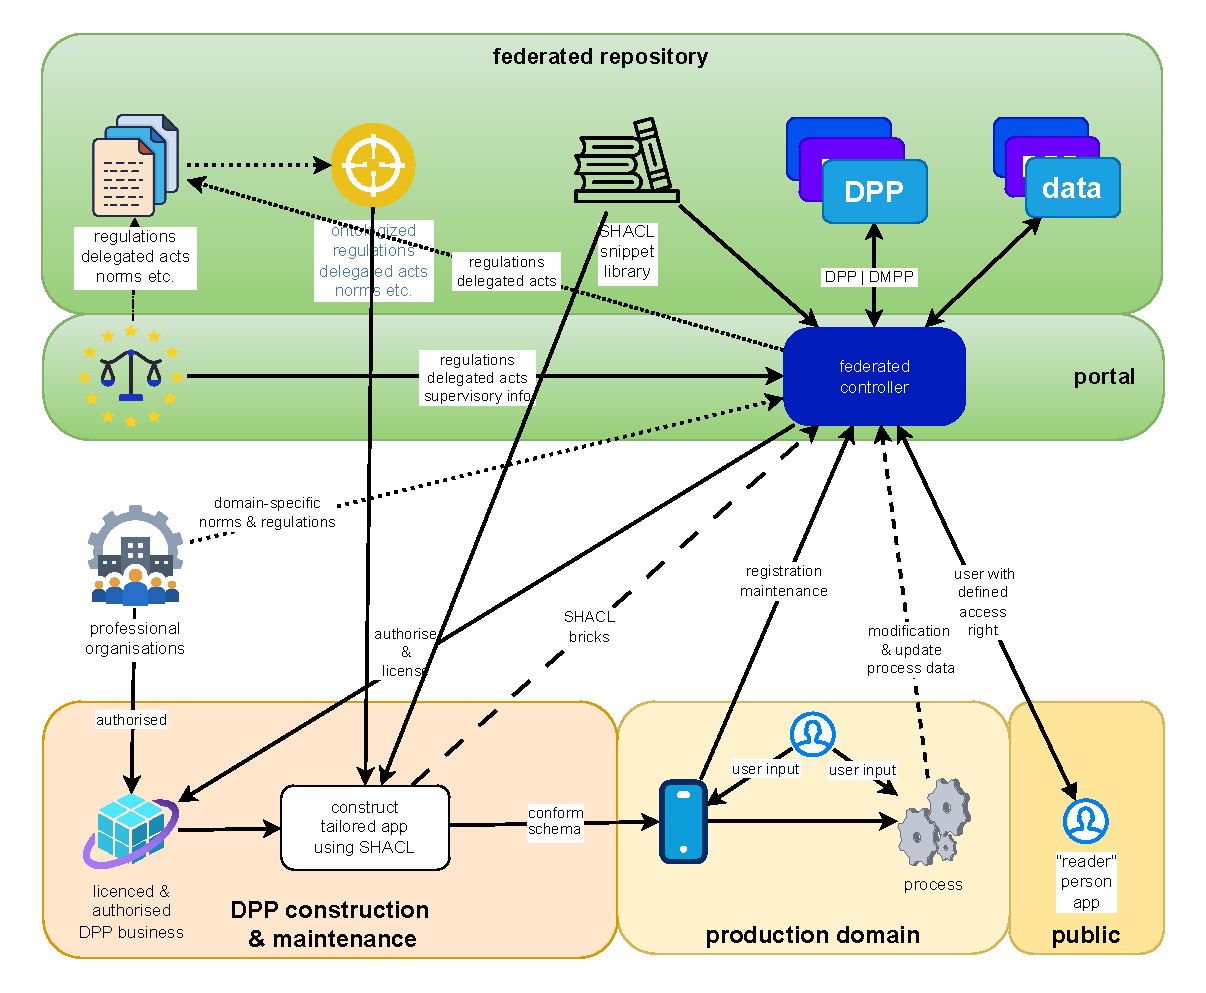
\includegraphics[width=0.9\linewidth]{figures/2025-10-16__DigiPass_DPP_handling-App-mech.pdf}
\caption{Conceptual overview of the portal-backed \DPP\ architecture. The federated repository (top) stores \DPP\ data, ontologised regulations, delegated acts, norms, and supervisory information. Professional organisations authorise and license \SHACL\ bricks, which are assembled into schemas for tailored app generation. The federated controller and portal (centre) govern access, modification rights, and updates. Licensed \DPP\ businesses construct tailored applications from the \SHACL\ schemas, ensuring that user-entered data conforms to regulations by construction. The ``reader'' person app provides public access to \DPP\ data.}
\label{fig:app-mech}
\end{figure}

This design places the responsibility for sustainable, long-term data custody with a clearly identifiable entity per jurisdiction --- the national portal operator --- rather than dispersing it across hundreds of thousands of \EROs\ whose operational continuity cannot be guaranteed over the decades-long lifespan envisioned for \DPP\ data. Each national portal instance is not merely a registry that maps identifiers to external endpoints; it is the authoritative repository of the \DPP\ data for economic operators registered in that jurisdiction. The \EC\ central registry, whose implementing act was identified by the European Commission representative at \DPPforEU~2026 as the first piece of legislation to be adopted~\cite{dpp4eu2026_day1}, provides the identifier resolution and regulatory framework, while the portal provides the data storage and governance layer. The two are complementary: the registry points to the portal, and the portal serves the data.

\subsection{Federation of National Portals}

The federated portal model envisions one portal per \EU\ member state, each behaving identically in terms of \API, data model, and access governance, but operating on data relevant to economic operators registered in that jurisdiction. Thus, the portal is not a single central server: it is a federation of interoperable national portals, each storing and governing the \DPP\ data of economic operators registered in its jurisdiction. This federation addresses sovereignty concerns while maintaining architectural uniformity. A common portal specification provides a unified architectural baseline that proactively addresses the emergence of parallel approaches across jurisdictions, as called for by a JTC~24 conference participant.

\subsection{The Ingestion Governance Loop}

When an \REO\ submits \DPP\ data to the portal, the data passes through an \textbf{Ingestion Governance Loop} --- a sequence of validation, normalisation, and storage operations performed by the portal controller before the data is committed to the triple-store. This loop ensures that all ingested \DPPs\ are semantically valid, cryptographically authenticated, and normalised to canonical ontological entities before they become queryable.

\subsubsection{SHACL Validation}

The first stage of ingestion is validation against \SHACL\ shapes. \SHACL\ (Shapes Constraint Language) is a W3C standard for describing and validating \RDF\ graphs against a set of structural constraints called ``shapes.'' The portal controller maintains a library of \SHACL\ shapes --- one set for each product category and applicable regulation --- and validates every submitted \DPP\ against the shapes corresponding to its product type and regulatory context. If validation fails, the \DPP\ is rejected with a structured error report indicating which shapes were violated and which data points failed. 
This design directly addresses the conference observation that machine-readable product data must become checkable by machine-readable regulation (see Section~6.2 for a detailed discussion of \SHACL\ conformity checking).
The portal-backed architecture makes this a present capability by hosting both the \DPP\ data and the \SHACL\ validation shapes in a unified triple-store within each national portal instance, enabling automated compliance checking at ingestion time.

\subsubsection{Cryptographic Alignment}

Each submitted \DPP\ must be cryptographically signed by the \REO\ that authored it. The portal controller verifies the signature against the \REO's registered public key, which is bound to the \REO's identity through the trust tier matrix (Section~5). This ensures that only authenticated, authorised economic operators can submit \DPP\ data to the portal. The cryptographic signature also provides non-repudiation: once a \DPP\ is submitted and signed, the \REO\ cannot deny authorship of the data. While the conference discussion on data carrier verification focused on verifying the physical carrier (e.g., \QR\ code on a product)~\cite{dpp4eu2026_day1}, the portal-backed architecture extends verification to the data layer itself: every \DPP\ in the triple-store is cryptographically authenticated.

\subsubsection{External Entity Normalisation}

\DPP\ data frequently references external entities: chemical substances (identified by \CAS\ numbers or \EC\ numbers), standards (identified by standard numbers), certifiers (identified by accreditation body identifiers), and materials (identified by various classification schemes). The portal controller normalises these references to canonical \IRIs\ using a set of external registry lookup services. For example, a reference to a chemical substance submitted as ``CAS 7440-44-0'' is normalised to a canonical \IRI\ such as \texttt{urn:echa:substance:7440-44-0}, linking it to the \ECHA\ database entry for that substance. This normalisation ensures that all \DPPs\ in the triple-store use consistent, resolvable identifiers for external entities, enabling cross-\DPP\ queries (e.g., ``find all products containing this substance'') to execute correctly. This design is grounded in the conference observation that the \DPP\ must link to standards, measurements, and certificates through the quality infrastructure~\cite{dpp4eu2026_day1}.

\subsection{The Resolution Governance Loop}

When a user (consumer, professional, circular operator, or authority) requests \DPP\ data from the portal, the request passes through a \textbf{Resolution Governance Loop} --- a sequence of authentication, authorisation, graph slicing, and serialisation operations performed by the portal controller before the data is returned to the requester. This loop ensures that each user sees only the data branches they are authorised to access.

\subsubsection{Authentication and Authorisation}

The requester is first authenticated via the \EC\ Authorisation App (Section~5.6), which leverages \eIDAS~2.0 digital identity wallets to establish the requester's identity. The requester's attributes (user category, jurisdiction, organisational affiliation, certifications) are then evaluated against the \ODRL\ access policies attached to each branch of the requested \DPP. This step implements the \ABAC\ framework described in Section~5. The conference observation from the battery passport context --- that the actor should see only ``\textit{those data that he's allowed to see but nothing more}''~\cite{dpp4eu2026_day2} --- is precisely the behaviour implemented by this stage.

\subsubsection{Graph Slicing via Dynamic \SPARQL\ CONSTRUCT}

Once the requester's access rights are determined, the portal controller constructs a \textbf{filtered sub-graph} of the requested \DPP\ --- a view that contains only the data branches the requester is authorised to see. This is implemented as a dynamic \SPARQL\ \texttt{CONSTRUCT} query: the controller generates a query that traverses the \DPP's named graph, selects only the triples whose attached \ODRL\ policies permit access for the requester's attributes, and constructs a new \RDF\ graph containing only the authorised triples. The resulting filtered graph is then serialised in the requested format (\JSONLD, \TURTLE, \RDF/ \XML) and returned to the requester. This approach --- dynamic, query-time filtering rather than pre-computed views --- ensures that access policies can be updated without regenerating stored views, and that the most current policy is always applied.

\subsubsection{Link Traversal Within the Portal}

When the filtered \DPP\ is returned to the requester, it may contain \texttt{dpp:hasPrecursor} and \texttt{dpp:derivedFrom} links to other \DPPs\ within the portal. The requester may then request those linked \DPPs, which pass through the same Resolution Governance Loop. Critically, because all linked \DPPs\ reside within the same portal triple-store, link traversal never produces \texttt{404 Not Found} errors (unless a \DPP\ has been explicitly revoked). The link rot problem --- identified in Section~2 as a systemic risk of the distributed model --- is structurally eliminated. This architectural design directly answers the data persistency concern raised in Section~2.1: data persists because it is stored in a governed repository, not at an unmanaged endpoint.

\subsection{Relationship to the \EC\ Central Registry}

The portal-backed architecture is complementary to, not competitive with, the \EC\ central registry. The registry provides:

\begin{itemize}
\item \textbf{Identifier resolution}: mapping product unique identifiers (as defined in EN~18215 \cite{en18215}) to portal endpoints.
\item \textbf{Regulatory metadata}: hosting the \SHACL\ shape library and ontologised regulations (Section~6).
\item \textbf{Public key infrastructure}: registering \REO\ public keys for cryptographic verification.
\item \textbf{Audit and compliance}: logging portal operations for regulatory oversight.
\end{itemize}

The portal provides:

\begin{itemize}
\item \textbf{Data storage}: hosting \DPP\ named graphs in a per-member-state triple-store.
\item \textbf{Ingestion governance}: \SHACL\ validation, cryptographic alignment, entity normalisation.
\item \textbf{Resolution governance}: \ABAC-based graph slicing, \SPARQL\ CONSTRUCT filtering.
\item \textbf{Link traversal}: resolving \texttt{dpp:hasPrecursor} and \texttt{dpp:derivedFrom} within the portal.
\end{itemize}

This division of responsibility resolves the tension observed at \DPPforEU~2026, where the Materials Commons initiative acknowledged that it does not ``\textit{run servers in the end}''~\cite{dpp4eu2026_day2}. The portal-backed architecture fills this gap: it runs the servers, stores the data, and governs access, while the \EC\ central registry provides the identifier, regulatory, and oversight layer.

\subsection{The Public Repository for Ontologised Regulations and Standards}

A critical component of the portal architecture is a \textbf{public repository 
for ontologised regulations and standards}, hosted on the \EC\ \DPP\ registry 
alongside the \SHACL\ shape library. This repository contains machine-readable 
representations of legal requirements, delegated acts, and harmonised 
standards that apply to each product category. The conference principle that 
``\textit{everything needs to be ontologized}''~\cite{dpp4eu2026_day2} is 
realised through this repository: regulations, standards, data models, and 
validation shapes are all represented as semantic, machine-readable artefacts 
within a unified framework. Section~6 discusses the public repository, the 
\SHACL\ brick library, and the two-stage design toolchain in detail.


\subsection{The Portal \API}

The portal exposes a standardised \REST\ \API\ that enables economic operators and application developers to interact with the portal controller programmatically. As a conference participant emphasised at \DPPforEU~2026~\cite{dpp4eu2026_day1}, the \API\ should cover ``\textit{all major business cases of registering... first of creating a digital product passport, being able to update it being able to delete or revoke it and then finally to register it with the European Commission's \DPP\ registry}''. A standardised \API\ is essential because, as another participant observed~\cite{dpp4eu2026_day1}, ``\textit{the implementation of an \API\ creates no unique selling point for anyone}'' and leaving \API\ implementation to small teams is ``\textit{already too much for them}''. The portal \API\ aligns with the \JTC~24 \API\ module (EN~18222~\cite{en18222}) and the Asset Administration Shell \API\ specifications~\cite{dpp4eu2026_day1}, which are ``\textit{already in review and publicly accessible}''~\cite{dpp4eu2026_day2}.

The portal \API\ is organised around five operation groups corresponding to the \DPP\ lifecycle:

\begin{enumerate}
\item \textbf{Authentication}: The requester presents an \eIDAS~2.0 digital identity credential to the \EC\ Authorisation App (Section~5.6), which returns a short-lived bearer token containing the requester's attributes (user category, organisation, jurisdiction, certifications).
\item \textbf{\DPP\ Lifecycle Management}: Authenticated \REOs\ can create, read, update, revoke, and register \DPPs. Each operation passes through the Ingestion Governance Loop (Section~4.2) for \SHACL\ validation, cryptographic alignment, and external entity normalisation before the \DPP\ is committed to the triple-store.
\item \textbf{\DPP\ Resolution}: Authenticated users can request a \DPP\ by its unique identifier. The request passes through the Resolution Governance Loop (Section~4.3), which evaluates \ODRL\ policies against the requester's attributes and returns a filtered sub-graph containing only the authorised branches.
\item \textbf{Link Traversal}: Authenticated users can request linked \DPPs\ by following \texttt{dpp:hasPrecursor} and \texttt{dpp:derivedFrom} links returned in a resolved \DPP. Each linked \DPP\ request passes through the same Resolution Governance Loop.
\item \textbf{\SPARQL\ Query}: Advanced users (professional users, circular operators, market surveillance authorities) can submit \SPARQL\ queries against the portal's triple-store. The portal controller executes the query with dynamic \ODRL-based graph filtering, returning only triples from branches the requester is authorised to access.
\end{enumerate}

The full \API\ specification, including endpoint paths, \HTTP\ methods, request and response schemas, and authentication flows, is provided in Appendix~\ref{app:api-spec}. Example interaction sequences covering the five operation groups are provided in Appendix~\ref{app:api-examples}.

% ===================================================================
\section{\ABAC\ Framework and \ODRL\ Access Policies}
% ===================================================================

\subsection{The Need for Granular Access Control}

The \ESPR\ mandates that \DPPs\ serve multiple user categories with different information needs and access rights. A consumer scanning a \QR\ code on a product needs access to public-facing information about composition, repairability, and environmental impact. A professional user --- a repair technician, a product designer, or a supply chain partner --- needs access to technical specifications and component data. A circular economy operator --- a recycler or a remanufacturer --- needs access to detailed material composition and hazard data. A market surveillance authority needs access to compliance documentation and full supply chain provenance. The Responsible Economic Operator (REO) who authored the \DPP\ needs access to the complete data record, including proprietary formulation details. The distributed flat-file model does not inherently support this granularity: an \ERO\ endpoint either serves the complete \DPP\ payload or a subset, but without a formal framework for attribute-based, branch-level filtering. As a representative from the battery passport context described at the \DPPforEU~2026 conference (see Section~1.4), the requirement is that the actor is authenticated and authorised so that they see only the data they are permitted to access --- nothing more. This is precisely the behaviour that the Attribute-Based Access Control (\ABAC) framework presented in this section implements, following the \NIST\ Attribute-Based Access Control definition~\cite{abac_nist} adapted to the \DPP\ context.

\subsection{Five Standardised User Categories}

We define five standardised user categories within the \DPP\ access governance framework, each with a distinct set of attributes, permissions, and authentication requirements.

\subsubsection{\texttt{dpp:PublicUser}}

The public user category encompasses consumers and any individual accessing \DPP\ data without formal organisational affiliation. Access is limited to public-facing data branches: product name, basic composition summary, environmental impact indicators, repairability information, and recycling instructions. Authentication is lightweight --- the \EC\ Authorisation App verifies the request origin but does not require organisational identity. No sensitive commercial data, supply chain details, or proprietary formulations are exposed to this category.

\subsubsection{\texttt{dpp:ProfessionalUser}}

The professional user category encompasses repair technicians, product designers, supply chain partners, and other economic operators with a legitimate professional interest in the product's \DPP\ data. Access includes technical specifications, component identifiers, supplier information (at the organisational level), and compliance documentation. Authentication requires organisational identity verification through the trust tier matrix (Section~5.5). Access is granted on a need-to-know basis~\cite{dpp4eu2026_day1}, reflecting the conference observation that professional users ``\textit{will never get the full access or they shouldn't get the full access}'' to all data in the \DPP~\cite{dpp4eu2026_day1}.

\subsubsection{\texttt{dpp:CircularOperator}}

The circular operator category encompasses recyclers, remanufacturers, and waste management operators who need detailed material composition, hazard classifications, and disassembly information to safely and effectively recover materials from end-of-life products. Access includes full composition data (including substances of concern), hazard statements, and disassembly instructions. Authentication requires both organisational identity and competence verification --- the operator must demonstrate that it is a legitimate circular economy actor with the appropriate certifications and authorisations for handling the materials in question. This category directly addresses the data persistency concern discussed in Section~2.1. The portal-backed architecture ensures that circular operators can access this data decades after manufacture, provided their credentials remain valid.

\subsubsection{\texttt{dpp:MarketSurveillanceAuthority}}

The market surveillance authority category encompasses national regulatory bodies responsible for verifying product compliance with applicable regulations. Access includes the full \DPP\ record: all data branches, all supply chain provenance, all compliance documentation, and all \REO\ declarations. Authentication requires governmental identity verification through \eIDAS~2.0 public sector identity credentials. This category has the broadest access rights, reflecting the regulatory mandate of market surveillance authorities under the ESPR. Full access is granted to authenticated regulatory bodies, and only to them, answering the conference question about who should have access to the full information~\cite{dpp4eu2026_day1}.

\subsubsection{\texttt{dpp:InternalDataOriginator}}

The internal data originator category encompasses the \REO\ that authored and submitted the \DPP. Access includes the complete \DPP\ record plus internal metadata: submission history, validation results, cryptographic signatures, and provenance logs. This category is unique in that it includes both the public and restricted data branches that the \REO\ authored, plus internal management data. Authentication requires the \REO's registered organisational identity and cryptographic key, bound through the trust tier matrix. This category enables the \REO\ to manage its own \DPPs: update data, correct errors, submit new versions, and monitor access logs.

\subsection{\ODRL\ Branch-Level Access Policies}

The \ABAC\ framework evaluates access decisions based on attributes of three entities: the \textbf{subject} (the requester, characterized by user category, organisational identity, jurisdiction, and certifications), the \textbf{object} (the \DPP\ data branch, characterized by its classification, sensitivity level, regulatory context, and applicable policies), and the \textbf{environment} (the request context, including time, jurisdiction, and active legal exceptions). This model follows the \NIST\ Attribute-Based Access Control definition~\cite{abac_nist}, adapted to the \DPP\ context. Access policies are encoded using the \WthreeC\ Open Digital Rights Language (\ODRL)~\cite{odrl_spec}, attached to individual branches within each \DPP's RDF named graph. Each data branch in a \DPP\ carries one or more \ODRL\ policies that specify which user categories may access it, under what conditions, and for what purposes. For example, a public-facing composition summary branch carries an \ODRL\ policy permitting access to all user categories. A proprietary formulation branch carries an \ODRL\ policy permitting access only to \\ \texttt{dpp:InternalDataOriginator} and \\ \texttt{dpp:MarketSurveillanceAuthority}. \\A supplier identity branch carries an \ODRL\ policy permitting access to \\ \texttt{dpp:ProfessionalUser}, \\ \texttt{dpp:CircularOperator}, \\ \texttt{dpp:MarketSurveillanceAuthority}, and \\ \texttt{dpp:InternalDataOriginator}, but not to \texttt{dpp:PublicUser}. \\ This branch-level policy attachment enables fine-grained access control that is not possible with binary, endpoint-level access models, directly addressing the conference concern about transferring confidential data only to authorised parties~\cite{dpp4eu2026_day1}.

\subsubsection{Example \ODRL\ Policy}

The following \ODRL\ policy, expressed in \JSONLD, attaches to a proprietary formulation branch within a \DPP, restricting access to the internal data originator and market surveillance authorities:

\begin{lstlisting}[language=jsonld]
{
  "@context": [
    "https://w3id.org/dpp/v1",
    "https://www.w3.org/ns/odrl.jsonld"
  ],
  "@type": "odrl:Policy",
  "odrl:permission": [
    {
      "odrl:action": "odrl:read",
      "odrl:target": "urn:dpp:product:batch-2026-001#formulation",
      "odrl:assignee": [
        {"@id": "dpp:InternalDataOriginator"},
        {"@id": "dpp:MarketSurveillanceAuthority"}
      ],
      "odrl:constraint": {
        "odrl:leftOperand": "dpp:regulatoryContext",
        "odrl:operator": "odrl:eq",
        "odrl:rightOperand": "ESPR"
      }
    }
  ]
}
\end{lstlisting}

This policy states that the \texttt{odrl:read} action on the formulation branch is permitted for \\ \texttt{dpp:InternalDataOriginator} and \\ \texttt{dpp:MarketSurveillanceAuthority} subjects, \\ provided the regulatory context is ESPR. The portal controller evaluates this policy during the Resolution Governance Loop (Section~4.3) when a requester attempts to access this branch.

\subsection{Dynamic \SPARQL\ CONSTRUCT Filtering}

The Resolution Governance Loop implements the \ABAC\ framework through dynamic \SPARQL\ \texttt{CONSTRUCT} queries. When a requester accesses a \DPP, the portal controller:

\begin{enumerate}
\item Authenticates the requester via the \EC\ Authorisation App (Section~5.6).
\item Retrieves the requester's attributes (user category, organisation, jurisdiction, certifications).
\item Retrieves the \DPP's named graph from the triple-store.
\item Evaluates the \ODRL\ policies attached to each data branch against the requester's attributes.
\item Constructs a filtered sub-graph containing only the branches for which the \ODRL\ evaluation returns \texttt{Permit}.
\item Serialises and returns the filtered graph to the requester.
\end{enumerate}

This dynamic, query-time filtering ensures that access policies are always evaluated against the most current \ODRL\ policies and the most current requester attributes. If a policy is updated (e.g., a new regulation expands circular operator access to additional data branches), the update takes effect immediately for all subsequent requests without requiring regeneration of stored views. The \SPARQL\ \texttt{CONSTRUCT} mechanism is well suited to this task because it operates natively on \RDF\ graphs and can express arbitrarily complex filtering conditions over both data and policy metadata.

\subsection{The Trust Tier Matrix}

Before a user can be assigned to one of the five categories and granted access to \DPP\ data, their identity and qualifications must be verified through a three-pillar trust tier matrix.

\subsubsection{Pillar 1: Legal Existence Verification}

The first pillar verifies that the organisation requesting access is a legally registered economic operator. This is performed through lookup in the European Economic Operators' Registration and Identification (EORI) system~\cite{eori_system} and the \VAT\ Information Exchange System (VIES)~\cite{vies_system}. The EORI number uniquely identifies an economic operator within the \EU\ customs and tax system, while \VIES\ confirms \VAT\ registration. 
\\
For a \texttt{dpp:MarketSurveillanceAuthority}, legal existence is verified through the governmental identity registry of the member state. 
\\
For a \texttt{dpp:PublicUser}, this pillar is not required (no organisational identity needed).

\subsubsection{Pillar 2: Competence Vetting}

The second pillar verifies that the organisation has the competence and certifications required for its claimed user category. 
\\
For a \texttt{dpp:CircularOperator}, this includes waste management permits, recycling certifications, and hazardous material handling authorisations. 
\\
For a \texttt{dpp:ProfessionalUser}, this includes professional qualifications relevant to the product category (e.g., electronics repair certification, automotive technician license). Competence is verified through \WthreeC\ Verifiable Credentials~\cite{verifiable_credentials} issued by accredited certification bodies. The verifiable credentials are cryptographically signed by the issuer, stored in the requester's \eIDAS~2.0 digital identity wallet, and presented to the portal controller during authentication. This pillar realises the quality infrastructure community's emphasis on linking \DPPs\ to standards, measurements, and certificates (see Section~7.4): certifications are verifiable credentials, and their provenance is traceable to the issuing accreditation body.

\subsubsection{Pillar 3: Identity Binding via \eIDAS\ 2.0}

The third pillar binds the organisational identity (Pillar~1) and the competence credentials (Pillar~2) to a verified natural person acting on behalf of the organisation. This is performed through \eIDAS~2.0~\cite{eidas2}, the European Digital Identity Framework, which provides a legally binding digital identity infrastructure across all \EU\ member states. The requester presents an \eIDAS~2.0 digital identity credential that links their natural person identity to their organisational role, and the portal controller verifies the binding. 
\\
For a \texttt{dpp:MarketSurveillanceAuthority}, the \eIDAS~2.0 credential confirms governmental authority. 
\\
For a \texttt{dpp:InternalDataOriginator}, the \eIDAS~2.0 credential confirms that the individual is authorised to submit \DPP\ data on behalf of the \REO. This three-pillar trust model ensures that access is granted only to verified organisations, with verified competence, acting through verified individuals --- a model that directly addresses the conference concern about data correctness and what is needed to prove that a data point is correct~\cite{dpp4eu2026_day1}.

\subsection{The \EC\ Authorisation App}

The authentication and authorisation pipeline is managed by an \EC\ Authorisation App, which serves as the centralised identity gatekeeper for the \DPP\ system. The app leverages \eIDAS~2.0 digital identity wallets to establish requester identity, retrieves organisational identity and competence credentials from the requester's wallet, and evaluates them against the trust tier matrix. Upon successful verification, the app issues a short-lived authorisation token containing the requester's attributes (user category, organisation, jurisdiction, certifications), which the portal controller uses to evaluate \ODRL\ policies during the Resolution Governance Loop. This centralised model ensures uniform authentication across all member state portals, consistent evaluation of trust tier requirements, and a single point of policy enforcement. The conference concern about data carrier verification and phishing~\cite{dpp4eu2026_day1} is addressed at the data access layer: only authenticated, authorised requesters can access \DPP\ data, and impersonation attempts are structurally prevented by the \eIDAS~2.0 identity binding.

\subsection{Resolving the \IP\ Leakage Risk}

The \ABAC\ framework with \ODRL\ branch-level policies directly resolves the intellectual property leakage risk identified in Section~2.4. In the distributed flat-file model, an \ERO\ endpoint serves the complete \DPP\ payload to any requester who reaches it, with no granular filtering. In the portal-backed model, the Resolution Governance Loop constructs a filtered sub-graph for each requester based on their attributes and the \ODRL\ policies attached to each branch. Proprietary formulation data, supplier identities, and process parameters are protected by \ODRL\ policies that restrict access to authorised user categories. A competitor who authenticates as a \texttt{dpp:ProfessionalUser} or \texttt{dpp:PublicUser} will see only the public and professional branches; the proprietary branches are filtered out by the \SPARQL\ \texttt{CONSTRUCT} query. The conference observation that ``\textit{this data really can be shared and if there's a compromise between confidentiality and transparency}''~\cite{dpp4eu2026_day1} is resolved by the \ABAC\ framework: the compromise is not a binary choice but a granular, policy-driven decision at the branch level. Each data branch can be independently classified, independently governed, and independently exposed or protected, based on the regulatory requirements and the commercial sensitivity of the data it contains. The transfer of intellectual property rights, identified as an open issue at the conference --- ``\textit{there's a transfer of \IPI. This is not covered yet in the standards because it's not quite clear how to organise this}''~\cite{dpp4eu2026_day1} --- can be modelled within this framework through \ODRL\ policies that specify \IPI-specific access conditions, updated dynamically as \IP\ rights transfer between organisations.

% ===================================================================%
% ===================================================================
\section{\SHACL\ as a Unified Data Modelling Language}
% ===================================================================

\subsection{The Dual Role of \SHACL}

A central innovation of the proposed architecture is the use of \SHACL\ (Shapes
Constraint Language)~\cite{shacl_spec} not merely as a validation tool but as a
\textbf{unified data modelling language} that serves two complementary purposes:
(1)~as the basis for conformity checking of submitted \DPP\ data against
applicable regulations and standards, and (2)~as the generative source for user
interfaces --- \DPP\ websites and application program interfaces --- via
\SHACL-to-HTML rendering engines. This dual role transforms \SHACL\ from a
passive validation layer into an active modelling substrate that drives both
data ingestion and data presentation.

At \DPPforEU~2026, \SHACL\ was described by a conference participant as
``\textit{a very elegant approach}'' for \DPP\ validation, and a NILU researcher
was introduced as speaking about ``\textit{\SHACL\ information models and how
they will be solving all our problems}''~\cite{dpp4eu2026_day1}. The conference
discussion revealed that the community recognises \SHACL's potential but has not
yet connected it to a portal-backed architecture where \SHACL\ shapes serve as
the single source of truth for both validation and interface generation. The
proposed architecture makes this connection explicit: \SHACL\ shapes are stored
in the public repository on the \EC\ \DPP\ registry, used by the portal
controller for ingestion validation (Section~4.2.1), and used by application
developers to generate user interfaces that, by construction, ensure
user-entered data conforms to regulations and standards.

\subsection{\SHACL\ for Conformity Checking}

The first role of \SHACL\ is conformity checking: verifying that submitted \DPP\
data satisfies the structural, cardinality, datatype, and semantic constraints
defined by applicable regulations and harmonised standards. As a \JTC~24
representative observed at \DPPforEU~2026, machine-readable product data must
become checkable by machine-readable regulation~\cite{dpp4eu2026_day1}. The
portal-backed architecture makes this a present capability by maintaining
\SHACL\ shapes --- one set for each product category and applicable regulation
--- in the same semantic framework as the \DPP\ data itself.

When an \REO\ submits \DPP\ data to the portal, the Ingestion Governance Loop
validates the data against the \SHACL\ shapes corresponding to the product's
category and regulatory context (Section~4.2.1). If validation fails, the \DPP\
is rejected with a structured error report indicating which shapes were violated
and which data points failed. This design ensures that only regulation-compliant
data enters the triple-store. The conformity checking is not a post-hoc audit
but a precondition for ingestion: data that does not conform to the applicable
\SHACL\ shapes is never committed to the portal.

The conference observation that ``\textit{you still have to look in the book
whether what you see on the screen is actually according to
requirements}''~\cite{dpp4eu2026_day1} is resolved structurally: the ``book''
(the regulation) is represented as \SHACL\ shapes, and the checking is performed
automatically at ingestion time. The quality infrastructure community's emphasis
on linking \DPPs\ to standards, measurements, and certificates (see Section~7.4)
is realised through \SHACL\ shapes that reference the applicable standards and
certificate schemas, ensuring that the \DPP\ data is not only structurally valid
but also semantically aligned with the regulatory requirements it claims to
satisfy.

\subsection{\SHACL\ for \GUI\ Generation via \DASH}

The second role of \SHACL\ is interface generation: using \SHACL\ shapes as the
basis for generating user interfaces --- web forms, mobile app screens, and
\API\ schemas --- that enable economic operators to enter \DPP\ data. This is
implemented through \SHACL-to-HTML rendering engines such as \DASH\ (\SHACL\
Application Dashboard)~\cite{dash_shacl} and the open-source shacl-form
library~\cite{shacl_form_lib} developed by the Universitäts- und
Landesbibliothek Darmstadt. At \DPPforEU~2026, a participant from the DigiPass
project described how \SHACL\ can ``\textit{validate a knowledge graph that is
coming as ingested information and it can also be used as has been done in our
project to automatically generate a form for manual data
ingest}''~\cite{dpp4eu2026_day2}.

This dual-use capability is the key insight: the same \SHACL\ shapes that
validate submitted data at the portal can also generate the data entry forms
that produce the data in the first place. When an application developer builds a
\DPP\ data entry tool --- a web platform or a mobile app --- they use the
\SHACL\ shapes from the public repository to generate the user interface. The
generated interface presents fields corresponding to the \SHACL\ properties,
enforces cardinality and datatype constraints, and validates user input against
the shapes in real time. By construction, the data entered through such an
interface conforms to the regulations and standards encoded in the \SHACL\
shapes. This eliminates the gap between data entry and data validation: the same
shapes govern both, ensuring that data is ``born compliant'' rather than being
checked for compliance after the fact.

\subsection{The \SHACL\ Brick Library}

To enable modular, maintainable, and regulation-aware interface generation, we
propose a \textbf{\SHACL\ brick library}: a collection of modular,
regulation-compliant \SHACL\ shape components --- ``bricks'' --- that are
reviewed against applicable regulations, delegated acts, and harmonised
standards, and then assembled into complete \SHACL\ schemas for specific product
categories and regulatory contexts.

A \SHACL\ brick represents a coherent unit of regulatory or standard-based
requirements: for example, a ``chemical composition brick'' that encodes the
data points and constraints required by \REACH\ for substance declaration, a
``carbon footprint brick'' that encodes the data points required by the ESPR for
environmental impact declaration, or a ``battery composition brick'' that
encodes the data points required by the Battery Regulation. Each brick is
independently developed, independently validated against the source regulation,
and independently versioned. When a new regulation is adopted, or an existing
regulation is amended, only the affected bricks are updated; all schemas that do
not use those bricks remain unchanged.

The brick library is hosted on the public repository for ontologised regulations
and standards (Section~6.7), making it accessible to all \DPP\ stakeholders:
portal operators, application developers, economic operators, and market
surveillance authorities. The conference principle that ``\textit{everything
needs to be ontologised}'' (Section~3.5) is realised through the brick library:
regulations, standards, data models, and validation shapes are all represented
as modular semantic artefacts within a unified framework.

\subsection{The Two-Stage \SHACL\ Design Toolchain}

The generation of complete \SHACL\ schemas from the brick library requires a
\textbf{two-stage \SHACL\ design toolchain}: a brick generator and a schema
assembler.

\subsubsection{Stage 1: The Brick Generator}

The brick generator is a tool that takes ontologised regulatory and
standard-based information as input and produces individual \SHACL\ bricks as
output. The input is domain-specific semantic information: ontologies,
vocabularies, and structured representations of regulatory requirements for a
specific product domain (e.g., batteries, textiles, construction products,
chemicals). The output is a set of \SHACL\ shape components, each encoding a
coherent unit of regulatory requirements. The brick generator requires that
semantic information for product-domain-specific regulations and standards be
generated and made available (Section~6.8). This is a non-trivial task: it
requires domain experts (regulatory specialists, standards experts, product
category specialists) to collaborate with ontology engineers to produce
machine-readable representations of regulatory requirements. The conference
discussion on building ``\textit{ontologies with
experts}''~\cite{dpp4eu2026_day2} directly motivates this stage: the brick
generator is the tool that bridges the gap between domain expert knowledge and
machine-readable \SHACL\ shapes.

\subsubsection{Stage 2: The Schema Assembler}

The schema assembler is a tool that takes a set of \SHACL\ bricks and assembles
them into a complete \SHACL\ schema for a specific product category and
regulatory context. The assembler selects the relevant bricks based on the
product category, the applicable regulations, and the applicable harmonised
standards, and combines them into a unified \SHACL\ shape graph. The assembled
schema is then used for two purposes: (1)~by the portal controller for ingestion
validation, and (2)~by application developers for interface generation via
\DASH\ or shacl-form. The assembler ensures that the assembled schema is
consistent --- no conflicting constraints, no duplicate properties, no missing
mandatory shapes --- and that it covers all regulatory requirements applicable
to the target product category. When a regulation is updated, the assembler
re-generates the schema from the updated bricks, ensuring that all downstream
applications --- portal validation, data entry forms, \API\ schemas --- reflect
the most current regulatory requirements.

\subsection{Licensed \DPP\ Application Ecosystem}
\label{sec:licensed-apps}

The \SHACL-driven architecture creates a new category of economic actor:
\textbf{licensed \DPP\ application providers} --- software businesses that
specialise in building, maintaining, and distributing regulation-compliant \DPP\
generation and maintenance applications for specific product domains. Rather
than monolithic \DPP\ platforms, these are lightweight, domain-specific
applications generated directly from the regulation-conformant \SHACL\ schemas
assembled by the schema assembler. For large
companies, the \DPP\ task may be handled as part of their internal
digitalisation programme; for smaller businesses, however, generating a \DPP\
can be very costly in terms of the time required to learn about the regulations
and delegated acts, and the process of registering and
maintenance~\cite{dpp4eu2026_postconf}. Licensed \DPP\ application providers
fill this gap by offering expertly designed software tools that run on small
computer systems, including PCs and mobile phones, handling the full \DPP\
lifecycle --- creation, registration, update, and maintenance --- without
requiring the economic operator to develop deep regulatory or semantic
expertise. As the DigiPass consortium envisioned, the approved \SHACL\ snippet
library serves as a very valuable source for generating such
applications~\cite{dpp4eu2026_postconf}.

\subsubsection{The Three-Stage Licensing Pipeline}

The generation of licensed \DPP\ applications extends the two-stage \SHACL\
design toolchain (Section~6.5) with a third stage: \textbf{app generation,
review, and licensing}. The full pipeline is:

\begin{enumerate}
\item \textbf{Brick generation} (Stage~1): domain experts and ontology engineers
produce \SHACL\ bricks from ontologised regulations and domain-specific semantic
information.
\item \textbf{Schema assembly} (Stage~2): the schema assembler combines bricks
into complete \SHACL\ schemas for specific product categories and regulatory
contexts.
\item \textbf{App generation and licensing} (Stage~3): licensed \DPP\
application providers construct tailored applications from the assembled \SHACL\
schemas, using \SHACL-to-HTML rendering engines such as \DASH\ or shacl-form.
The resulting application is reviewed, approved, and licensed for distribution.
\end{enumerate}

\subsubsection{Dual Authorisation}

The licensing of \DPP\ application providers follows a dual authorisation model,
reflecting the dual nature of the regulatory and professional requirements.
First, the \EC, through the portal authority, authorises the software business
to operate as a licensed \DPP\ application provider, verifying its legal
existence and operational competence. Second, professional organisations (e.g.,
industry associations, standardisation bodies) authorise the provider's
domain-specific competence, ensuring that the applications it produces are
technically and regulatorily appropriate for the product categories they cover.
This dual authorisation model mirrors the trust tier matrix (Section~5.5): legal
existence is verified through the first pillar, and domain competence is
verified through the second pillar, but applied to software providers rather
than data requesters.

\subsubsection{The Review Board}

A \textbf{review board} --- a technical body established at the authority/portal
level --- validates submitted \SHACL\ bricks, assembled schemas, and generated
applications against the applicable regulations, delegated acts, and
norms~\cite{dpp4eu2026_postconf}. The review board has three responsibilities:

\begin{enumerate}
\item \textbf{Brick review}: each \SHACL\ brick submitted to the public library
is reviewed for regulatory accuracy, semantic correctness, and consistency with
the source regulation.
\item \textbf{Schema review}: assembled \SHACL\ schemas are reviewed for
completeness (all applicable regulatory requirements covered), consistency (no
conflicting constraints), and correctness (no missing mandatory shapes).
\item \textbf{Application review}: generated \DPP\ applications are reviewed for
regulatory compliance, correct use of the portal \API, and foolproofness (see
Section~6.6.4).
\end{enumerate}

The review board is funded through a dedicated \EU\ budget line that finances
the maintenance of the open-access standards repository, the \SHACL\ brick
review process, and the federation-service \APIs~\cite{dpp4eu2026_postconf}.

\subsubsection{Foolproof by Construction}

The defining property of a licensed \DPP\ application is that it is
\textbf{foolproof by construction}: the application generates \RDF\ graphs that,
when submitted to the portal, will not fail \SHACL\ validation. This guarantee
is structural, not accidental. Because the application's data entry forms are
generated from the same \SHACL\ shapes that the portal controller uses for
ingestion validation (Section~4.2.1), the forms enforce exactly the constraints
that the portal will check. Cardinality, datatype, and semantic constraints are
validated in real time during data entry; the user cannot submit a \DPP\ that
violates a shape constraint because the form itself prevents it. As a conference
participant from the DigiPass project described, \SHACL\ can ``\textit{validate
a knowledge graph that is coming as ingested information and it can also be used
as has been done in our project to automatically generate a form for manual data
ingest}''~\cite{dpp4eu2026_day2}. The licensed \DPP\ application ecosystem
operationalises this dual-use capability as a guarantee: the same shapes that
validate at the portal generate the forms at the point of data entry, ensuring
that data is ``born compliant'' (Section~6.3). This is why the architecture
favours lightweight, domain-specific apps over monolithic platforms: only
applications generated from the same \SHACL\ shapes that govern portal ingestion
can offer a structural guarantee of compliance.

\subsubsection{Portal \API\ Integration}

Licensed \DPP\ applications must integrate with the portal \API\ (Section~4.6)
for all \DPP\ lifecycle operations: authentication, \DPP\ creation, update,
revocation, registration with the \EC\ central registry, link traversal, and
\SPARQL\ query. This requirement ensures that:

\begin{itemize}
\item All \DPP\ data generated by licensed applications passes through the
Ingestion Governance Loop, receiving \SHACL\ validation, cryptographic
alignment, and external entity normalisation.
\item All \DPP\ updates propagate correctly through the linked \DPP\ network via
\texttt{dpp:hasPrecursor} and \texttt{dpp:derivedFrom}.
\item All access requests pass through the Resolution Governance Loop, with
\ABAC\ policies enforced uniformly regardless of the originating application.
\end{itemize}

The portal \API\ thus serves as the single integration point between licensed
applications and the portal infrastructure, ensuring architectural consistency
across the entire application ecosystem.

\subsection{The Public Repository for Ontologised Regulations and Standards}

The brick library and the assembled \SHACL\ schemas are hosted in a
\textbf{public repository for ontologised regulations and standards}, maintained
on the \EC\ \DPP\ registry alongside the central identifier resolution service.
This repository contains:

\begin{itemize}
\item \textbf{Ontologised regulations}: machine-readable representations of the
ESPR, the Battery Regulation, \REACH, and product-specific delegated acts,
expressed as \RDF\ graphs with links to the original legal text.
\item \textbf{Ontologised standards}: machine-readable representations of
harmonised standards (EN~18215--18232 \cite{en18215}) and sector-specific
standards, expressed as \RDF\ graphs.
\item \textbf{\SHACL\ bricks}: modular shape components encoding regulatory and
standard-based requirements, produced by the brick generator.
\item \textbf{Assembled \SHACL\ schemas}: complete shape graphs for specific
product categories and regulatory contexts, produced by the schema assembler.
\item \textbf{Domain ontologies}: product-domain-specific ontologies (e.g.,
battery ontology, textile ontology, construction ontology) that provide the
semantic vocabulary for the \SHACL\ shapes.
\end{itemize}

The repository is public, freely accessible, and continuously updated as
regulations evolve and new product categories come under \DPP\ requirements. The
conference aspiration that standards should be ``\textit{publicly accessible,
and they should be for free, they should not be sold by \DIN\ and other
organisations}''~\cite{dpp4eu2026_day2} is operationalised through this
repository: ontologised regulations and standards are hosted on a public \EC\
infrastructure, accessible to all \DPP\ stakeholders without payment. Both the
regulations (as ontologised legal text) and the validation shapes (as \SHACL\
bricks and schemas) are available in machine-readable form, enabling automated
compliance checking at scale.

\subsection{Domain-Specific Semantic Information for Brick Generation}

The brick generator (Stage~1 of the toolchain) requires that semantic
information for product-domain-specific regulations and standards be generated
and made available. This is the foundational layer of the \SHACL\ architecture:
without domain-specific ontologies and structured regulatory representations,
the brick generator has no input, and no \SHACL\ bricks can be produced. As the
Materials Commons presentation at \DPPforEU~2026 described, this involves
``\textit{the implementation of the semantic framework network and the
infrastructure setup}''~\cite{dpp4eu2026_day2}.

The domain-specific semantic information must cover:

\begin{itemize}
\item \textbf{Regulatory requirements}: the specific data points, thresholds,
and constraints mandated by the ESPR, delegated acts, and product-specific
regulations for each product category.
\item \textbf{Standard-based requirements}: the specific data points,
measurement methods, and conformity assessment procedures defined by harmonised
standards (EN~18215--18232) \cite{en18215, en18216, en18217, en18221, en18222}
and sector-specific standards.
\item \textbf{Data models}: the structured representations of product,
component, and material data for each product category, including properties,
relationships, and cardinalities.
\item \textbf{Vocabularies}: the controlled vocabularies, code lists, and
classification schemes used in each product domain (e.g., material
classification codes, hazard categories, recycling codes).
\end{itemize}

This domain-specific semantic information is the input to the brick generator,
which produces \SHACL\ bricks that encode these requirements in a
machine-actionable form. The bricks are then assembled into complete schemas by
the schema assembler and published in the public repository, where they are
available for portal validation and interface generation.

\subsection{The SHACL-Driven Data Lifecycle}

The \SHACL-centric architecture creates a coherent data lifecycle that spans
from regulation to data entry to validation to storage to access:

\begin{enumerate}
\item \textbf{Regulation ontologisation}: regulations and standards are
represented as machine-readable semantic artefacts in the public repository.
\item \textbf{Brick generation}: the brick generator produces \SHACL\ bricks
from the ontologised regulations and domain-specific semantic information.
\item \textbf{Schema assembly}: the schema assembler combines bricks into
complete \SHACL\ schemas for specific product categories.
\item \textbf{Application generation and licensing}: licensed \DPP\ application
providers construct tailored applications from the assembled schemas, reviewed
and approved by the review board (Section~6.6).
\item \textbf{Data entry}: economic operators enter \DPP\ data through the
licensed applications, which validate input against the \SHACL\ shapes in real
time.
\item \textbf{Ingestion validation}: the portal controller validates submitted
\DPP\ data against the same \SHACL\ shapes during the Ingestion Governance Loop.
\item \textbf{Storage}: validated \DPP\ data is committed to the portal's
triple-store as \RDF\ named graphs.
\item \textbf{Access}: the Resolution Governance Loop filters and serves \DPP\
data based on \ABAC\ policies (Section~5).
\end{enumerate}

At every stage, the \SHACL\ shapes serve as the single source of truth for what
constitutes valid, regulation-compliant \DPP\ data, making the conference
aspirations for machine-checkable regulation and universal ontologisation
operational within a single, coherent architectural framework.

% ===================================================================
\section{Chemical Data Governance and Cross-Registry Linking}
% ===================================================================

\subsection{The Chemical Data Challenge}

A particularly challenging category of \DPP\ data is chemical composition and hazard information. The \ESPR, \REACH, the Battery Regulation, and product-specific delegated acts all require that \DPPs\ carry data on substances of concern, hazardous classifications, and material composition. However, this data category sits at the intersection of three structural tensions: (1)~the regulatory mandate for transparency, (2)~the commercial sensitivity of proprietary formulations, and (3)~the scientific authority of established chemical registries. A representative from the materials industry captured this tension directly at the \DPPforEU~2026 conference~\cite{dpp4eu2026_day2}, noting that the \DPP\ must address ``\textit{material safety, our chemical safety processes}'' while also acknowledging that there is ``\textit{a lot more that we need from this community in order to meet us in the middle}''. The distributed flat-file model resolves none of these tensions: it either exposes proprietary data or withholds it, and it either duplicates chemical hazard information from authoritative sources or omits it entirely.

\subsection{The Duplication Problem}

Chemical hazard data --- substance identities, hazard classifications, \SVHC\ listings, safety data sheet content --- is already maintained by authoritative public databases. The European Chemicals Agency (ECHA)~\cite{echa} maintains the authoritative registry of substances registered under \REACH, including \SVHC\ candidate list entries, harmonised classifications under \CLP, and authorisation list entries. \PubChem~\cite{pubchem} maintained by the U.S. National Library of Medicine provides open-access chemical substance information including structures, properties, and links to regulatory entries. Duplicating this data within individual \DPPs\ creates three problems. First, \textbf{data drift}: when ECHA updates a hazard classification or adds a substance to the \SVHC\ candidate list, all \DPPs\ that have duplicated the old classification become stale and inconsistent. Second, \textbf{scale}: with potentially millions of \DPPs\ across the European single market, each carrying duplicated chemical data, the storage and update burden becomes prohibitive. Third, \textbf{authority}: a hazard classification stated in a \DPP\ carries less authority than a classification linked to the ECHA database, because the \DPP\ data is self-declared by the \REO\ while the ECHA data is regulatorily authoritative.

\subsection{Cross-Registry Linking via External Entity Normalisation}

The portal-backed architecture resolves the duplication problem through the external entity normalisation stage of the Ingestion Governance Loop (Section~4.2.3). When an \REO\ submits a \DPP\ containing chemical substance references, the portal controller normalises these references to canonical \IRIs\ using external registry lookup services (e.g., ``\CAS\ 7440-44-0'' to \texttt{urn:echa:substance:7440-44-0}). The \DPP\ stores the \textit{link}, not the \textit{data}. When a user accesses the \DPP\ through the Resolution Governance Loop, the portal can resolve the link in real time, retrieving the current authoritative hazard classification from ECHA and presenting it alongside the \REO's composition declaration. This approach ensures that: (1)~the \DPP\ always reflects the most current authoritative hazard data, (2)~the storage burden is minimised (only links, not full data sets), and (3)~the authority of the data is preserved (it comes from ECHA, not from the \REO's self-declaration). The conference discussion on material declaration reinforced this principle, with a participant advocating for ``single point of definition'' (SPOD) --- ``\textit{one repository where we say that's how we identify a material and that are the definitions we serve to tell you what are the hazard statements what is the granularity}''~\cite{dpp4eu2026_day1}. The cross-registry linking approach operationalises the \SPOD\ principle within the portal-backed architecture.

\subsection{The Quality Infrastructure Connection}

The cross-registry linking strategy extends beyond chemical databases to the broader quality infrastructure: standards, measurements, and certificates. As a representative of the German quality infrastructure emphasised at the \DPPforEU~2026 conference~\cite{dpp4eu2026_day2}, the quality infrastructure ``\textit{allows to link the data from the \DPP\ to exactly those standards, measurements and certificates}'', with the further observation that certificate data could be directly implemented in the \DPP\ and that it is important to trace what standards were used to assess the information~\cite{dpp4eu2026_day2}. The portal-backed architecture realises this vision through external entity normalisation: when a \DPP\ references a standard (e.g., ``EN 18215''), a measurement (e.g., a specific test method), or a certificate (e.g., a conformity assessment certificate from an accredited body), the portal controller normalises these references to canonical \IRIs\ linking to the relevant quality infrastructure databases. The conference discussion also highlighted the importance of the quality infrastructure for trust: ``\textit{I think we have many \DPP\ proposals trying to make verifiable data without addressing, in particular, the QI, the quality infrastructure, and I think it's a waste of time because this is what we need to have in order to trust the \DPP\ structures at all}''~\cite{dpp4eu2026_day2}. The three-pillar trust tier matrix (Section~5.5) complements this by ensuring that the organisations providing certified data are themselves verified through \EORI\ / \VIES, \WthreeC\ Verifiable Credentials, and \eIDAS~2.0 identity binding.

\subsection{The \SVHC\ and \CLP\ Alignment}

A specific challenge is the representation of Substances of Very High Concern (SVHC) and harmonised classifications under the Classification, Labelling and Packaging (CLP) regulation in \DPPs. A conference participant from the materials manufacturing perspective noted at \DPPforEU~2026~\cite{dpp4eu2026_day1} that the industry needs consistency: ``\textit{if we talk about \SVHCs, follow the same definition from \CLP\ and the candidate list from ECHA whether you work in textiles, automotive tyres, or furniture}''. The cross-registry linking approach ensures this consistency structurally: rather than each \REO\ defining \SVHC\ and \CLP\ classifications independently in their \DPPs, all \DPPs\ link to the same ECHA-maintained candidate list and \CLP\ harmonised classification entries. When ECHA adds a substance to the \SVHC\ candidate list, all \DPPs\ containing that substance automatically reflect the updated status upon resolution, without requiring any action from the \REOs. This design directly addresses the conference concern about consistency and eliminates the risk of divergent \SVHC\ classifications across product categories.

\subsection{The Industry Dilemma: Proprietary Composition and Partial Disclosure}

A well-documented tension in \DPP\ implementation is the resistance of chemical and materials companies to disclosing proprietary composition data through a system that could expose it to competitors. The conference discussion on confidential data sharing~\cite{dpp4eu2026_day1} exemplifies this concern. The \ABAC\ framework with \ODRL\ branch-level policies (Section~5) provides the architectural answer: proprietary composition branches are protected by \ODRL\ policies that restrict access to 
\\
\texttt{dpp:InternalDataOriginator} and 
\\
\texttt{dpp:MarketSurveillanceAuthority}, 
\\
while public-facing composition summaries (which may omit proprietary details) are accessible to \texttt{dpp:PublicUser}. The cross-registry linking strategy adds a further dimension: for hazard classification data that is already public in ECHA, the \DPP\ can link to ECHA rather than duplicating the classification, allowing the public to see the hazard information without the \REO\ disclosing its proprietary formulation. The \REO\ declares the presence of the substance (and links to its ECHA entry) without disclosing the exact quantity or formulation context. This partial disclosure model --- link to public hazard data, protect proprietary composition --- resolves the Industry dilemma within a single architectural framework. The conference observation that ``\textit{this data really can be shared and if there's a compromise between confidentiality and transparency}''~\cite{dpp4eu2026_day1} is realised through this granular, branch-level approach.

\subsection{Interoperability with Industry Data Platforms}

The cross-registry linking strategy must also address interoperability with industry-specific data platforms that already maintain chemical and materials data. A conference presentation demonstrated interoperability between ChemX and ContainerX at the Hannover Messe, where ``\textit{SECA as a client picked up the data from Covestro that was polymer data}''~\cite{dpp4eu2026_day2}. The portal-backed architecture supports such interoperability through external entity normalisation: when a \DPP\ references a material from an industry platform (e.g., a Covestro polymer grade), the portal controller normalises the reference to a canonical \IRI\ that links to the industry platform's entry for that material. This design accommodates both public registries (ECHA, \PubChem) and industry platforms (ChemX, Materials Commons), treating them uniformly as external authoritative sources that \DPPs\ link to rather than duplicate. The Materials Commons initiative (Section~2.2) serves as one such external source. The portal-backed architecture complements Materials Commons by providing the storage, access governance, and ingestion validation that Materials Commons explicitly does not offer.

\subsection{The Open-Source Material Characterisation Database}

A conference participant described at \DPPforEU~2026~\cite{dpp4eu2026_day1} the development of ``\textit{an open-source database with the material characterisation for everybody to have access to identifiers for free and also to test material compositions}''. This initiative aligns with the cross-registry linking strategy: open-access material characterisation databases can serve as additional external authoritative sources that \DPPs\ link to. The portal controller's external entity normalisation can accommodate multiple registries --- ECHA for regulatory hazard data, \PubChem\ for chemical substance information, open-source material characterisation databases for materials property data --- normalising all references to canonical \IRIs\ and resolving them in real time during the Resolution Governance Loop. This multi-registry approach ensures that \DPPs\ carry the most authoritative, most current, and most comprehensive data available, without duplicating any of it.

% ===================================================================
\section{Discussion}
% ===================================================================

\subsection{Beyond Compliance: \DPP\ as Business Enabler}

A recurring theme at \DPPforEU~2026 was the need to ensure that \DPPs\ are perceived and implemented as more than a regulatory compliance burden. As a conference speaker emphasised at \DPPforEU~2026~\cite{dpp4eu2026_day3}, the goal is to ``\textit{make sure that the implementation and the perception of \DPPs\ stay beyond compliance}''. The portal-backed architecture supports this transition: by hosting \DPPs\ as queryable knowledge graphs in a centralised triple-store, the portal enables not only compliance checking but also advanced use cases --- supply chain analytics, circular economy business model innovation, AI-driven material recovery optimisation, and cross-product substance tracking --- that go far beyond the minimum regulatory requirements. The conference observation that \DPPs\ should ``\textit{transit from statistic documentation to the intelligent decision support system}''~\cite{dpp4eu2026_day3} is directly enabled by the portal's \SPARQL-queryable knowledge graph architecture, which transforms static \DPP\ records into a living, queryable substrate for circular economy intelligence.

\subsection{The Governance Challenge: Human Agreement, Not Technology}

A striking post-conference reflection from the DigiPass \CSA\ project crystallised a conclusion that emerged across the event: the \DPP\ challenge is fundamentally one of governance and human agreement, not technology. As Peter Klein, the DigiPass \CSA\ project leader, wrote in the post-conference summary~\cite{dpp4eu2026_postconf}:

\begin{quote}\emph{
``All the excellent presentations, posters, and podium discussions at the \DPPforEU\ crystallized one particular conclusion in my mind: the solution of the \DPP\ challenge is more related to human agreement, commitment, and collaboration than to any technical implementation issue.''
}
\end{quote}

This observation was echoed by Paul Breiner of the TRUSTex project, who described the conference's value as ``\textit{the transdisciplinary exchange of technical, regulatory, governance and industry-related perspectives around a common objective: unlocking the Digital Product Passport's potential to drive the systemic transition towards a Circular Economy}''~\cite{dpp4eu2026_postconf}. The portal-backed architecture proposed in this paper is fundamentally a governance architecture: it provides the structural framework within which human agreement, commitment, and collaboration can be operationalised. The portal is not a technological endpoint; it is the institutional infrastructure that makes cross-organisational data governance possible at scale.

\subsection{The Role of DigiPass Europe as Community Sustainer}

The conference revealed a clear aspiration within the DigiPass consortium to sustain the community beyond the \CSA's lifetime. As a speaker noted at \DPPforEU~2026~\cite{dpp4eu2026_day2}, the plan is to ``\textit{go from DigiPass to DigiPass Europe}'' in order to ``\textit{create a community around these topics that sustain the effort that has been made so far with everyone}''. The proposed portal-backed architecture aligns with this aspiration: DigiPass Europe could serve as the organisational entity that operates or oversees the federated portal infrastructure, the public repository for ontologised regulations, and the \SHACL\ brick library. The conference observation that ``\textit{we need actually for this to act a kind of central hub connecting the industry the stakeholders}''~\cite{dpp4eu2026_day2} maps directly onto the portal's role as the semantic and governance hub of the \DPP\ ecosystem. The \COST\ action model, described as a bottom-up initiative open to all interested participants~\cite{dpp4eu2026_day2}, provides a complementary funding and governance mechanism for the ongoing community work, particularly for the domain-specific semantic information generation that the \SHACL\ brick library requires.

The conference format itself --- a single-track, ``one-for-all'' programme deliberately designed to avoid community fragmentation --- reflects the same architectural principle underlying the portal-backed model. As Heinz Adolf Preisig observed in the post-conference summary: ``\textit{One could argue for separate sessions and longer talks, but it would split the community. Given the status of the \DPP\ development affair, I felt a need to see the complete picture and minimise the formation of specialised groups}''~\cite{dpp4eu2026_postconf}. The architectural parallel is direct: just as the conference community resisted fragmentation through a unified

% ===================================================================
\section{Conclusion and Roadmap}
% ===================================================================

\subsection{Summary of Contributions}

This paper has proposed a portal-backed, graph-based, network-structured \DPP\
architecture built on semantic web standards that addresses the systemic
vulnerabilities of the current distributed, flat-file model. The architecture
comprises six integrated components: (1)~the Networked Individual \DPP\ model
with semantic linking properties (\texttt{dpp:hasPrecursor},
\texttt{dpp:derivedFrom}), in which each \DPP\ is a knowledge graph node in a
production network; (2)~the portal as semantic proxy archive, storing all \DPP\
data --- including \REO\ product data --- behind a federation of national
portals, one per \EU\ member state; (3)~an \ABAC\ framework with five
standardised user categories and ODRL branch-level access policies, ensuring
strictly controlled, granular access for protection of sensitive data; (4)~a
three-pillar trust tier matrix combining \EORI\ / \VIES, \WthreeC\ Verifiable
Credentials, and \eIDAS~2.0; (5)~\SHACL\ as a unified data modelling language
serving both conformity checking and \GUI\ generation, supported by a \SHACL\
brick library, a two-stage design toolchain, a licensed \DPP\ application
ecosystem with dual authorisation and review board, and a public repository for
ontologised regulations and standards; and (6)~a cross-registry linking strategy
for chemical data governance, connecting \DPPs\ to authoritative public
databases rather than duplicating data. Evidence from the \DPPforEU~2026
conference --- comprising 150 in-person participants, over 1,700 online
participants, and representatives of four European Commission
Directorate-Generals, HaDEA, and CEN/CENELEC \JTC~24~\cite{dpp4eu2026_postconf}
--- demonstrates that the constituent elements of this architecture are
independently recognised as necessary by the practitioner community. This paper
integrates them into a coherent whole.

\subsection{The Roadmap for the European Commission}

The proposed architecture aligns with a vision already anticipated within the
DigiPass consortium. An internal consortium deliverable anticipated a future in
which ``\textit{there is indeed a European \DPP\ Registry with: registration,
\API\ access, semantic repository}'' --- a vision that maps directly onto the
portal-backed architecture proposed here~\cite{dpp4eu2026_postconf}. The
European Commission's funding agency has likewise recognised the need for
structural coordination: Giuseppe Giovanni Daquino of HaDEA observed at
\DPPforEU~2026 that the agency ``\textit{clearly identified how these projects
are clustered through the \DPP\ connection with SSbD processes and its
integration and strategic alignment with the European advanced materials
innovation ecosystem}''~\cite{dpp4eu2026_postconf}. The federated portal
architecture provides exactly this clustering and integration function at the
technical level.

Based on the architecture proposed in this paper, we recommend the following
roadmap for the European Commission:

\subsubsection{Phase 1 (2026--2027): Foundation}

\begin{itemize}
\item Adopt the federated portal specification as the architectural baseline for
the \DPP\ central registry infrastructure, complementing the identifier
resolution function with the portal's data storage and governance layer.
\item Establish the public repository for ontologised regulations and standards
on the \EC\ \DPP\ registry, beginning with the ESPR, the Battery Regulation, and
\REACH.
\item Pilot the portal architecture with the first product category (batteries),
using the Battery Regulation requirements as the initial \SHACL\ shape library.
\item Begin the \SHACL\ brick generation process for the battery domain,
engaging domain experts and ontology engineers.
\item Establish the review board for \SHACL\ bricks, schemas, and licensed \DPP\
applications, with a dedicated \EU\ budget line for ongoing maintenance.
\item Define the dual authorisation framework for licensing \DPP\ application
providers, involving both the European Commission and relevant professional
organisations.
\end{itemize}

\subsubsection{Phase 2 (2027--2028): Expansion}

\begin{itemize}
\item Extend the portal architecture to the next product categories (textiles,
construction products, electronics), generating domain-specific \SHACL\ brick
libraries for each.
\item Begin licensing the first \DPP\ application providers for the battery
domain, using the \SHACL\ schemas produced in Phase~1.
\item Deploy the federated portal across all willing \EU\ member states, with a
common specification and interoperability testing.
\item Integrate the three-pillar trust tier matrix with the \EC\ Authorisation
App, leveraging \eIDAS~2.0 digital identity wallets.
\item Begin cross-registry linking implementation, starting with ECHA for
chemical hazard data and expanding to other quality infrastructure databases.
\item Expand the licensed application ecosystem to textiles, construction
products, and electronics as domain-specific \SHACL\ brick libraries become
available.
\end{itemize}

\subsubsection{Phase 3 (2028--2030): Maturation}

\begin{itemize}
\item Achieve full federated portal coverage across all \EU\ member states.
\item Complete the \SHACL\ brick library for all priority product categories
under the ESPR.
\item Establish the DigiPass Europe community entity as the ongoing custodian of
the \SHACL\ brick library and the domain-specific semantic information, with
\COST\ action or equivalent funding.
\item Extend the cross-registry linking strategy to industry data platforms
(Materials Commons, ChemX, sector-specific platforms).
\item Explore extension of the portal specification to non-\EU\ countries for
global \DPP\ interoperability through UN/CEFACT and \ISO/\IEC\ \JTC~5.
\end{itemize}

\subsection{The Path Forward}

The conference chair's closing observation --- that ``\textit{this year's
conference was very inspiring. It has stronger results. It has clearer
contributions, a deeper understanding of what the passport is and what it could
yet become}''~\cite{dpp4eu2026_day3} --- captures the moment. The \DPP\
community has reached a point of clarity about what is needed: semantic
representations, persistent storage, granular access control, quality
infrastructure integration, machine-readable regulation, and a licensed
application ecosystem that makes compliance accessible to enterprises of all
sizes. What is missing is the integrated architecture that combines these
elements. This paper proposes such an architecture. The path forward requires
the European Commission, member states, standards bodies, and the practitioner
community to collaborate on its implementation --- a collaboration that the
DigiPass Europe initiative, the \COST\ action, and the \JTC~24/\JTC~5
standardisation processes are well positioned to sustain.



\section*{acknowledgments}
This work is being funded by the EC's Horizon Europe research and
innovation programme, we acknowledge GA no.~101138510 (DigiPass CSA).


\section*{Declaration on Generative AI}
The author(s) have not employed any Generative AI tools for analysing the conference transcripts, the post-conference report, and proofreading. 

\appendix
% ===================================================================
\appendix
\section{Portal API Specification}
\label{app:api-spec}
% ===================================================================
\setcounter{table}{0}

This appendix specifies the portal \REST\ \API. All endpoints use HTTPS with TLS
1.3. Request and response bodies are \JSON\ (for management operations) or
\JSONLD\ / \TURTLE\ / \RDF\ / \XML\ (for \DPP\ data). All requests except
authentication require a valid bearer token in the \texttt{Authorization}
header.

\subsection{Authentication}

\begin{table}[h]
\centering
\caption{Authentication endpoint.}
\label{tab:api-auth}
\begin{tabular}{p{0.2\textwidth} p{0.2\textwidth} p{0.55\textwidth}}
\toprule
\textbf{Method} & \textbf{Path} & \textbf{Description} \\
\midrule
POST & \texttt{/auth/token} & Exchange \eIDAS\ 2.0 credential for a bearer
token. Returns a short-lived JWT containing the requester's attributes. \\
\bottomrule
\end{tabular}
\end{table}

\textbf{Request body} (\JSON):
\begin{lstlisting}[language=json,breaklines=true,breakatwhitespace=true]
{
  "eidasCredential": "<\eIDAS 2.0 digital identity credential>",
  "requestedScopes": ["dpp:read", "dpp:write"]
}
\end{lstlisting}

\textbf{Response body} (JSON):
\begin{lstlisting}[language=json,breaklines=true,breakatwhitespace=true]
{
  "accessToken": "<JWT>",
  "tokenType": "Bearer",
  "expiresIn": 3600,
  "attributes": {
    "userCategory": "dpp:ProfessionalUser",
    "organisation": "urn:eori:DE123456789",
    "jurisdiction": "DE",
    "certifications": ["urn:vc:electronics-repair-cert"]
  }
}
\end{lstlisting}

\subsection{\DPP\ Lifecycle Management}

\begin{table}[h]
\centering
\caption{\DPP\ lifecycle management endpoints.}
\label{tab:api-lifecycle}
\small
\begin{tabular}{p{0.10\textwidth} p{0.30\textwidth} p{0.60\textwidth}}
\toprule
\textbf{Method} & \textbf{Path} & \textbf{Description} \\
\midrule
POST & \texttt{/dpps} & Submit a new \DPP. The request body is a signed JSON-LD
document. Passes through the Ingestion Governance Loop. Returns the assigned
\DPP\ \URI and validation report. \\
\addlinespace
GET & \texttt{/dpps/\{dppId\}} & Retrieve a \DPP\ by its unique identifier.
Passes through the Resolution Governance Loop. Returns a filtered JSON-LD
sub-graph based on the requester's access rights. \\
\addlinespace
PUT & \texttt{/dpps/\{dppId\}} & Update an existing \DPP. The request body is a
signed JSON-LD document with the updated content. Requires
\texttt{dpp:InternalDataOriginator} role. Triggers re-validation through the
Ingestion Governance Loop. \\
\addlinespace
DELETE & \texttt{/dpps/\{dppId\}} & Revoke a \DPP. The \DPP\ is marked as
revoked (not physically deleted; provenance is preserved). Requires
\texttt{dpp:InternalDataOriginator} role. \\
\addlinespace
POST & \texttt{/dpps/\{dppId\}/register} & Register a \DPP\ with the EC central
registry. Maps the \DPP\ \URI to the product unique identifier in the EC
registry. Requires \texttt{dpp:InternalDataOriginator} role. \\
\bottomrule
\end{tabular}
\end{table}

\textbf{POST /dpps --- Request body} (JSON-LD):
\begin{lstlisting}[language=jsonld,%
breaklines=true,%
breakatwhitespace=true,%
columns=fullflexible]
{
  "@context": "https://w3id.org/dpp/v1",
  "@id": "urn:dpp:product:batch-2026-001",
  "@type": "dpp:ProductPassport",
  "dpp:productName": "Lithium-Ion Battery Pack Model X",
  "dpp:hasPrecursor": [...],
  "dpp:derivedFrom": {...},
  "dpp:signature": {
    "algorithm": "RS256",
    "value": "<base64-encoded signature>",
    "certificate": "<X.509 certificate URI>"
  }
}
\end{lstlisting}

\textbf{POST /dpps --- Response body} (\JSON):
\begin{lstlisting}[language=json,%
breaklines=true,%
breakatwhitespace=true,%
columns=fullflexible]
{
  "dppId": "urn:dpp:product:batch-2026-001",
  "status": "accepted",
  "validationReport": {
    "shaclConformant": true,
    "cryptographicVerified": true,
    "entitiesNormalized": 14,
    "errors": []
  }
}
\end{lstlisting}

\textbf{GET /dpps/\{dppId\} --- Response body} (\JSONLD, filtered):
\begin{lstlisting}[language=jsonld,%
breaklines=true,%
breakatwhitespace=true,%
columns=fullflexible]
{
  "@context": "https://w3id.org/dpp/v1",
  "@id": "urn:dpp:product:batch-2026-001",
  "@type": "dpp:ProductPassport",
  "dpp:productName": "Lithium-Ion Battery Pack Model X",
  "dpp:hasPrecursor": [
    {"@id": "urn:dpp:component:cathode-b789"},
    {"@id": "urn:dpp:component:anode-b456"}
  ],
  "dpp:filteredBranches": ["dpp:public", "dpp:professional"]
}
\end{lstlisting}

Note: The \texttt{dpp:filteredBranches} property is a metadata annotation added
by the portal controller to indicate which branches were included in the
response, enabling the client to understand what was filtered out.

\subsection{Link Traversal}

\begin{table}[h]
\centering
\caption{Link traversal endpoint.}
\label{tab:api-links}
\small
\begin{tabular}{p{0.10\textwidth} p{0.35\textwidth} p{0.55\textwidth}}
\toprule
\textbf{Method} & \textbf{Path} & \textbf{Description} \\
\midrule
GET & \texttt{/dpps/\{dppId\}/precursors} & Retrieve all precursor \DPPs\ linked
via \texttt{dpp:hasPrecursor}. Each linked \DPP\ is resolved through the
Resolution Governance Loop and returned as a filtered subgraph. \\
\addlinespace
GET & \texttt{/dpps/\{dppId\}/derivations} & Retrieve all derivation \DPPs\
linked via \texttt{dpp:derivedFrom}. Each linked \DPP\ is resolved through the
Resolution Governance Loop and returned as a filtered sub-graph. \\
\addlinespace
GET & \texttt{/dpps/\{dppId\}/supplychain} & Recursively traverse the full
supply chain by following \texttt{dpp:hasPrecursor} and \texttt{dpp:derivedFrom}
links. Returns an aggregated \JSONLD\ graph containing all accessible linked
\DPPs, each filtered according to the requester's access rights. \\
\bottomrule
\end{tabular}
\end{table}

\subsection{\SPARQL\ Query}

\begin{table}[h]
\centering
\caption{\SPARQL\ query endpoint.}
\label{tab:api-sparql}
\small
\begin{tabular}{p{0.10\textwidth} p{0.15\textwidth} p{0.75\textwidth}}
\toprule
\textbf{Method} & \textbf{Path} & \textbf{Description} \\
\midrule
POST & \texttt{/sparql} & Submit a \SPARQL\ CONSTRUCT or SELECT query. The
portal controller executes the query with dynamic ODRL-based graph filtering:
only triples from branches the requester is authorised to access are returned.
The response is returned in the requested serialisation format (\JSONLD,
\TURTLE, \RDF\ / \XML, or \SPARQL\ \JSON results). \\
\bottomrule
\end{tabular}
\end{table}

\textbf{Request body} (\JSON):
\begin{lstlisting}[language=json,%
breaklines=true,%
breakatwhitespace=true,%
columns=fullflexible]
{
  "query": "CONSTRUCT { ?s ?p ?o } \
    WHERE { ?s ?p ?o . \
      ?s dpp:containsSubstance \
      <urn:echa:substance:7440-44-0> }",
  "format": "application/ld+json"
}
\end{lstlisting}

\textbf{Response body} (\JSONLD, filtered by access rights):
\begin{lstlisting}[language=jsonld,%
breaklines=true,%
breakatwhitespace=true,%
columns=fullflexible]
{
  "@context": "https://w3id.org/dpp/v1",
  "@graph": [
    {
      "@id": "urn:dpp:product:batch-2026-001",
      "dpp:containsSubstance":
        {"@id": "urn:echa:substance:7440-44-0"},
      "dpp:productName":
        "Lithium-Ion Battery Pack Model X"
    }
  ]
}
\end{lstlisting}

\subsection{Error Handling}

All error responses use standard HTTP status codes and a consistent \JSON\ error
body:

\begin{table}[h]
\centering
\caption{Error response codes.}
\label{tab:api-errors}
\small
\begin{tabular}{p{0.12\textwidth} p{0.25\textwidth} p{0.58\textwidth}}
\toprule
\textbf{Code} & \textbf{Meaning} & \textbf{Description} \\
\midrule
400 & Bad Request & The request body is malformed, or the \SHACL\ validation
failed. The response includes a structured validation report. \\
\addlinespace
401 & Unauthorised & The bearer token is missing, expired, or invalid. \\
\addlinespace
403 & Forbidden & The requester's attributes do not permit access to the
requested resource or branch. \\
\addlinespace
404 & Not Found & The requested \DPP\ does not exist or has been revoked. \\
\addlinespace
409 & Conflict & The \DPP\ already exists (on POST) or has been modified since
retrieval (on PUT). \\
\addlinespace
422 & Unprocessable Entity & The \DPP\ is semantically valid JSON-LD but fails
\SHACL\ validation. The response includes the \SHACL\ validation report. \\
\bottomrule
\end{tabular}
\end{table}

\textbf{Error response body} (JSON):
\begin{lstlisting}[language=json,%
breaklines=true,%
breakatwhitespace=true,%
columns=fullflexible]
{
  "error": {
    "code": "SHACL_VALIDATION_FAILED",
    "message": "The submitted DPP does not conform \
      to the applicable SHACL shapes.",
    "validationReport": [
      {
        "shape": "dpp:BatteryCompositionShape",
        "property": "dpp:carbonFootprint",
        "constraint": "sh:minCount",
        "value": 0,
        "expected": 1
      }
    ]
  }
}
\end{lstlisting}

\clearpage
% ===================================================================
\section{Example API Interaction Sequences}
\label{app:api-examples}
% ===================================================================

This appendix provides concrete examples of \API\ interactions covering the five
operation groups defined in Section~4.6.

\subsection{Example 1: \REO\ Submits a New \DPP}

An economic operator (EO) submits a new \DPP\ for a battery batch. The
interaction proceeds as follows:

\begin{enumerate}
\item \textbf{Authenticate}: The \EO\ presents its \eIDAS~2.0 credential to
obtain a bearer token.
\item \textbf{Submit DPP}: The \EO\ submits the signed \JSONLD\ \DPP\ via POST
\texttt{/dpps}.
\item \textbf{Ingestion}: The portal controller validates the \DPP\ against
\SHACL\ shapes, verifies the cryptographic signature, normalises external entity
references, and commits the \DPP\ to the triple-store.
\item \textbf{Register}: The \EO\ registers the \DPP\ with the EC central
registry via POST \texttt{/dpps/\{dppId\}/register}.
\end{enumerate}

\begin{lstlisting}[language=bash,breaklines=true,breakatwhitespace=true]
# Step 1: Authenticate
curl -X POST https://portal.example.eu/auth/token \
  -H "Content-Type: application/json" \
  -d '{"eidasCredential": "...",
       "requestedScopes": ["dpp:write"]}'

# Response: {"accessToken": "<JWT>", "attributes": {...}}

# Step 2: Submit DPP
curl -X POST https://portal.example.eu/dpps \
  -H "Authorization: Bearer <JWT>" \
  -H "Content-Type: application/ld+json" \
  -d @dpp-batch-2026-001.jsonld

# Response: {"dppId": "urn:dpp:product:batch-2026-001",
#            "status": "accepted",
#            "validationReport": {...}}

# Step 3: Register with EC central registry
curl -X POST \
  https://portal.example.eu/dpps/\
urn:dpp:product:batch-2026-001/register \
  -H "Authorization: Bearer <JWT>"

# Response: {"registryStatus": "registered",
#            "productIdentifier": \
#            "EN18215:DE:123456789:batch-2026-001"}
\end{lstlisting}

\subsection{Example 2: Consumer Scans \QR\ Code and Reads Public \DPP}

A consumer scans a \QR\ code on a product and requests the public-facing \DPP\
data. The interaction proceeds as follows:

\begin{enumerate}
\item \textbf{Authenticate}: The consumer's app presents a lightweight
\eIDAS~2.0 credential (no organisational identity required) to obtain a
\texttt{dpp:PublicUser} bearer token.
\item \textbf{Resolve \DPP}: The consumer's app requests the DPP via GET
\texttt{/dpps/\{dppId\}}.
\item \textbf{Filter}: The portal controller evaluates ODRL policies against the
\texttt{dpp:PublicUser} attributes and returns only the public-facing branches
(product name, basic composition summary, environmental impact indicators,
repairability information, recycling instructions).
\end{enumerate}

\begin{lstlisting}[language=bash,breaklines=true,breakatwhitespace=true]
# Step 1: Authenticate (lightweight)
curl -X POST https://portal.example.eu/auth/token \
  -H "Content-Type: application/json" \
  -d '{"eidasCredential": "...",
       "requestedScopes": ["dpp:read"]}'

# Response: {"accessToken": "<JWT>",
#            "attributes": {
#              "userCategory": "dpp:PublicUser", ...}}

# Step 2: Resolve DPP
curl -X GET \
  https://portal.example.eu/dpps/\
urn:dpp:product:batch-2026-001 \
  -H "Authorization: Bearer <JWT>" \
  -H "Accept: application/ld+json"

# Response: JSON-LD with only public-facing branches
# (dpp:filteredBranches: ["dpp:publicBranch"])
\end{lstlisting}

\subsection{Example 3: Circular Operator Traverses Supply Chain}

A certified recycler needs the full material composition and disassembly
information for a product at end-of-life. The interaction proceeds as follows:

\begin{enumerate}
\item \textbf{Authenticate}: The recycler presents its \eIDAS~2.0 credential
(including waste management permits and recycling certifications as \WthreeC\
Verifiable Credentials) to obtain a \texttt{dpp:CircularOperator} bearer token.
\item \textbf{Resolve \DPP}: The recycler requests the \DPP via GET
\texttt{/dpps/\{dppId\}}. The portal returns a filtered sub-graph including the
full composition data, hazard statements, and disassembly instructions.
\item \textbf{Traverse Supply Chain}: The recycler requests the full supply
chain via GET \texttt{/dpps/\{dppId\}/supplychain}. The portal recursively
follows \texttt{dpp:hasPrecursor} links and returns an aggregated JSON-LD graph
containing all accessible precursor \DPPs, each filtered according to the
recycler's access rights.
\end{enumerate}

\begin{lstlisting}[language=bash,breaklines=true,breakatwhitespace=true]
# Step 1: Authenticate
curl -X POST https://portal.example.eu/auth/token \
  -H "Content-Type: application/json" \
  -d '{
    "eidasCredential": "...",
    "verifiableCredentials": [
      "urn:vc:waste-mgmt-permit-DE-123",
      "urn:vc:recycling-cert-EU-456"
    ],
    "requestedScopes": ["dpp:read"]
  }'

# Response: {"accessToken": "<JWT>",
#            "attributes": {
#              "userCategory": "dpp:CircularOperator",
#              ...}}

# Step 2: Resolve DPP
curl -X GET \
  https://portal.example.eu/dpps/\
urn:dpp:product:batch-2026-001 \
  -H "Authorization: Bearer <JWT>" \
  -H "Accept: application/ld+json"

# Response: JSON-LD with composition, hazard,
#   and disassembly branches
# (dpp:filteredBranches: ["dpp:public",
#   "dpp:composition", "dpp:hazard",
#   "dpp:disassembly"])

# Step 3: Traverse full supply chain
curl -X GET \
  https://portal.example.eu/dpps/\
urn:dpp:product:batch-2026-001/supplychain \
  -H "Authorization: Bearer <JWT>" \
  -H "Accept: application/ld+json"

# Response: Aggregated JSON-LD graph with all
#   accessible precursor DPPs
\end{lstlisting}

\subsection{Example 4: Market Surveillance Authority Runs Cross-Product \SPARQL\
Query}

A market surveillance authority needs to identify all products in the portal
that contain a specific substance of concern. The interaction proceeds as
follows:

\begin{enumerate}
\item \textbf{Authenticate}: The authority presents its \eIDAS~2.0 governmental
credential to obtain a \texttt{dpp:MarketSurveillanceAuthority} bearer token.
\item \textbf{\SPARQL\ Query}: The authority submits a \SPARQL\ CONSTRUCT query
via POST \texttt{/sparql} that traverses all \DPPs\ in the portal and identifies
those containing the target substance. The portal controller executes the query
with full access rights (no \ODRL\ filtering for market surveillance
authorities) and returns the aggregated result.
\end{enumerate}

\begin{lstlisting}[language=bash,breaklines=true,breakatwhitespace=true]
# Step 1: Authenticate
curl -X POST https://portal.example.eu/auth/token \
  -H "Content-Type: application/json" \
  -d '{"eidasCredential": "<gov credential>",
       "requestedScopes": ["dpp:read","dpp:sparql"]}'

# Response: {"accessToken": "<JWT>",
#            "attributes": {
#              "userCategory": "dpp:MarketSurveillance",
#              ...}}

# Step 2: SPARQL query
curl -X POST https://portal.example.eu/sparql \
  -H "Authorization: Bearer <JWT>" \
  -H "Content-Type: application/json" \
  -d '{
    "query": "CONSTRUCT { ?dpp \
        dpp:containsSubstance ?substance . \
        ?dpp dpp:productName ?name } \
      WHERE { ?dpp \
        dpp:containsSubstance \
        <urn:echa:substance:7440-44-0> . \
        ?dpp dpp:productName ?name }",
    "format": "application/ld+json"
  }'

# Response: JSON-LD graph with all DPPs
#   containing the target substance
\end{lstlisting}

\subsection{Example 5: \REO\ Updates a \DPP\ After a Hazard Reclassification}

\ECHA\ reclassifies a substance, adding it to the \SVHC\ candidate list. The
\REO\ of a product containing that substance updates the \DPP\ to reflect the
new classification. The interaction proceeds as follows:

\begin{enumerate}
\item \textbf{Authenticate}: The \REO\ presents its \eIDAS~2.0 credential to
obtain a \texttt{dpp:InternalDataOriginator} bearer token.
\item \textbf{Retrieve \DPP}: The \REO\ retrieves the current \DPP\ via GET
\texttt{/dpps/\{dppId\}} (with full access rights as the data originator).
\item \textbf{Update \DPP}: The \REO\ submits the updated \DPP\ via PUT
\texttt{/dpps/\{dppId\}} with the corrected substance reference (now linking to
the updated \ECHA\ entry via the normalised \IRI). The portal controller
re-validates the \DPP\ against \SHACL\ shapes, verifies the signature, and
commits the updated version to the triple-store. All parent product \DPPs\ that
reference this \DPP\ via \texttt{dpp:hasPrecursor} automatically reflect the
updated classification upon subsequent resolution.
\end{enumerate}

\begin{lstlisting}[language=bash,breaklines=true,breakatwhitespace=true]
# Step 1: Authenticate
curl -X POST https://portal.example.eu/auth/token \
  -H "Content-Type: application/json" \
  -d '{"eidasCredential": "...",
       "requestedScopes": ["dpp:read","dpp:write"]}'

# Response: {"accessToken": "<JWT>",
#            "attributes": {
#              "userCategory": "dpp:InternalDataOriginator",
#              ...}}

# Step 2: Retrieve current DPP
curl -X GET \
  https://portal.example.eu/dpps/\
urn:dpp:product:batch-2026-001 \
  -H "Authorization: Bearer <JWT>" \
  -H "Accept: application/ld+json"

# Step 3: Update DPP with corrected substance ref
curl -X PUT \
  https://portal.example.eu/dpps/\
urn:dpp:product:batch-2026-001 \
  -H "Authorization: Bearer <JWT>" \
  -H "Content-Type: application/ld+json" \
  -d @dpp-batch-2026-001-updated.jsonld

# Response: {"dppId": "urn:dpp:product:batch-2026-001",
#            "status": "updated",
#            "validationReport": {...},
#            "version": 2}
\end{lstlisting}

\clearpage

\bibliographystyle{plain}
\bibliography{references}

\end{document}